\documentclass[a4paper,11pt]{article}
\usepackage[utf8]{inputenc}

%   Castellano
\usepackage[spanish,english,activeacute]{babel}
\decimalpoint
\usepackage{boxedminipage}

%lorem
\usepackage{lipsum}

%   Matemáticas
\usepackage{ucs}
\usepackage{amsfonts}
\usepackage{amssymb}
\usepackage[T1]{fontenc}
\usepackage{amsmath}
\usepackage{lmodern}
\usepackage[margin=4cm]{geometry}
\usepackage{resizegather} %Para ecuaciones muy largas

%Import the natbib package and sets a bibliography  and citation styles
\usepackage{natbib}
\bibliographystyle{abbrvnat}
% \bibliographystyle{plain}
\setcitestyle{authoryear}
% \setcitestyle{authoryear,open={((},close={))}}
\usepackage{enumerate}
\usepackage{ftnxtra}

%footnote pegado a la zona inferior de la pagina
\usepackage[bottom]{footmisc}

%   Figuras
\usepackage{graphicx}
\DeclareGraphicsExtensions{.bmp,.pdf,.png,.jpg,.gif,.jpeg}
\usepackage[mathscr]{eucal}
\usepackage[nottoc]{tocbibind}
\usepackage[colorlinks,urlcolor=blue,citecolor=blue,linkcolor=blue,filecolor=blue]{hyperref}
\usepackage{subfig}

%Cambia espaciado tablas
\usepackage{setspace}

\usepackage{svg}

%   Tablas
%\usepackage{colortbl}% color
\usepackage{lscape}% vertical
% \usepackage{multirow}

% Tablas avanzadas
\usepackage{fancyhdr}
\markboth{izquierdo}{derecho}
\usepackage{pgfplotstable,array,booktabs}

% \usepackage{listings}

\usepackage{textcomp}

%   Programación
\usepackage{minted}
\usepackage{etoolbox}

\newmintedfile[mybash]{bash}{
    linenos=true,
    breaklines=true,
    encoding=utf8,
    fontsize=\footnotesize,
    frame=lines
}

% \newmintedfile[mybash]{bash}{
%     linenos,
%     numbersep=4pt,
%     encoding=utf8,
%     gobble=0,
%     frame=lines,
%     framesep=2mm,
% }

\newmintedfile[mypython]{python}{
    linenos,
    numbersep=5pt,
    encoding=utf8,
    gobble=0,
    frame=lines,
    framesep=2mm,
}

%%%%
%Arbol directorios
\usepackage{tikz}
\usetikzlibrary{trees}

\usepackage{xcolor}
\tikzstyle{every node}=[thick,anchor=west, rounded corners, font={\scriptsize\ttfamily}, inner sep=2.5pt]
\tikzstyle{selected}=[draw=blue,fill=blue!10]
\tikzstyle{root}=[selected, fill=blue!30]
%%%%


% Cambiar formato de una sola pagina
\usepackage{geometry}

%   Para introducir páginas en blanco
\usepackage{afterpage}

\usepackage[toc,page]{appendix}

%   formato del documento
%   Formato de las páginas
% altura cabecera
\setlength{\headheight}{1 pt}
% distancia cabecera caja
\setlength{\headsep}{20 pt}
% separación entre el pie y la caja
\setlength{\footskip}{10 mm}
% paperheight=margen superior, margen inferior 
\setlength{\textheight}{\dimexpr\paperheight-1.5 cm-\headheight-\headsep-\footskip-1 cm}
\setlength{\topmargin}{\dimexpr 1cm-1in}
% anchura pagina, margenes laterales
\setlength{\textwidth}{\dimexpr \paperwidth-1.75cm*2}
\setlength{\oddsidemargin}{\dimexpr 1.75cm-1in}

\usepackage[left=1.5cm,top=2.5cm,right=1.5cm,bottom=2.5cm]{geometry} 

%Interlineado
\renewcommand{\baselinestretch}{1.3}

% \usepackage[left=1.5cm,top=2.5cm,right=1.5cm,bottom=2.5cm]{geometry} 

% \usepackage{geometry}
%  \geometry{
%  a4paper,
%  total={170mm,257mm},
%  left=20mm,
%  top=15mm,
%  right=25mm,
%  bottom=20mm
%  }

%   Comandos definidos por el usuario
%    NUEVOS COMANDOS DEFINIDOS MEDIANTE NEWCOMAND
\DeclareMathOperator\erf{erf}

% ENTORNO MATEMÁTICO
\newcommand{\maths}[1]{$ #1 $}

% TEXTO RESALTADO
\newcommand{\resalta}[1]{\textit{#1}}
\newcommand{\anglicismo}[1]{\textit{#1}}
\newcommand{\cultismo}[1]{\textit{#1}}
\newcommand{\comillas}[1]{``#1''}

% SÍMBOLOS MATEMÁTICOS
\newcommand{\menoroigual}{$\geqslant$}
\newcommand{\delorden}{$\sim$}
\newcommand\norm[1]{\left\lVert#1\right\rVert}
\newcommand{\porcentaje}[1]{$#1\:\%$}

%\lesssim  	less or quivalent
% \gtrsim 

% UNIDADES
%   PROPIAS DE ASTRONOMÍA
\newcommand{\solares}[2]{$#2 \:{#1}_{\odot}$}
\newcommand{\masassolares}[1]{$#1 \:{M}_{\odot}$}
\newcommand{\luminosidadessolares}[1]{$#1 \:{L}_{\odot}$}
\newcommand{\tfe}[1]{$#1 \:{M}_{\odot}\,\mathrm{{yr}^{-1}}$}
% \newcommand{\myr}{}
\newcommand{\flujo}[1]{${S}_{#1 \:\mu\mathrm{m}}$}
%   GENERALES
\newcommand{\microm}[1]{$#1 \:\mu\mathrm{m}$}
\newcommand{\angstrom}[1]{$#1 \:$\AA}
\newcommand{\mjy}[1]{$#1 \:\mathrm{mJy}$}
\newcommand{\jy}[1]{$#1 \:\mathrm{Jy}$}
\newcommand{\kelvin}[1]{$#1 \:\mathrm{K}$}
%   Grados celsius
\newcommand{\grad}{$^{\circ}$}

% NOMBRES USADOS FRECUENTEMENTE
\newcommand{\hatlas}{\mbox{\textit{H}-ATLAS}}
\newcommand{\halos}{\mbox{HALOS}}
\newcommand{\halo}{\mbox{HALO}}
\newcommand{\gama}{\mbox{GAMA}}
\newcommand{\spire}{\mbox{SPIRE}}
\newcommand{\pacs}{\mbox{PACS}}
\newcommand{\hifi}{\mbox{HIFI}}
\newcommand{\h}{\textit{\mbox{Herschel}}}
\newcommand{\rt}{\textit{\mbox{redshift}}}
\newcommand{\rts}{\textit{\mbox{redshifts}}}
\newcommand{\sed}{\mbox{SED}}
\newcommand{\sfr}{\mbox{SFR}}
\newcommand{\slg}{\mbox{SLG}}
\newcommand{\etg}{\mbox{ETG}}
\newcommand{\cross}{\mbox{cross-identificación}}
\newcommand{\smm}{\mbox{SMM~J2135-0102}}
\newcommand{\arp}{\mbox{Arp220}}
\newcommand{\gquince}{\mbox{G15.141}}

\newcommand{\typewriter}[1]{\texttt{#1}}
\newcommand{\python}{\texttt{\mbox{Python}}}
\newcommand{\script}{\textit{\mbox{script}}}

% PARÁMETROS
\newcommand{\z}{\textit{z}}
\newcommand{\paramk}{'K'}
\newcommand{\paramc}{'C'}

%   Compuestos químicos
\newcommand{\agua}{H_{2}O}

%   Nuevos comandos para tablas
%http://tex.stackexchange.com/questions/12703/how-to-create-fixed-width-table-columns-with-text-raggedright-centered-raggedlef
\newcolumntype{L}[1]{>{\raggedright\let\newline\\\arraybackslash\hspace{0pt}}m{#1}}
\newcolumntype{C}[1]{>{\centering\let\newline\\\arraybackslash\hspace{0pt}}m{#1}}
\newcolumntype{R}[1]{>{\raggedleft\let\newline\\\arraybackslash\hspace{0pt}}m{#1}}

%   Modificación de la linea para el pie de página
%https://es.wikibooks.org/wiki/Manual_de_LaTeX/Gestionando_la_bibliograf%C3%ADa/Notas_al_pie
\renewcommand{\footnoterule}{\vspace*{-3pt}
  \noindent\rule{5cm}{1pt}\vspace*{2.6pt}}
  
% densidad del cultivo
\newcommand{\rhocultivo}{\mbox{${\rho}_c$}}
% densidad de la muestra
\newcommand{\rhomuestra}{\mbox{${\rho}_c$}}

% celulas/mm3
\newcommand{\celpormmcubico}[1]{$cel {mm}^{-3}$}
% celulas/ml
\newcommand{\celporml}{\hspace{-0,5mm}$\mathrm{cel {ml}^{-1}}$}
% micrometros
\newcommand{\micrometro}{\hspace{-0,5mm}$\mathrm{\mu m}$}
% microlitros
\newcommand{\microlitro}{\hspace{-0,5mm}$ \mathrm{\mu l}$}
% picolitros
\newcommand{\picolitro}{\hspace{-0,5mm}$\mathrm{pl}$}
% litro
\newcommand{\litro}{\hspace{-0,5mm}$\mathrm{l}$}
% Grados Celsius
\newcommand{\celsius}{\hspace{-2,5mm}$\phantom{a}^{\circ} \mathrm{C}$}
% Omios
\newcommand{\ohm}{\hspace{-0,5mm}$\Omega$}
% KiloOmios
\newcommand{\kiloohm}{\hspace{-0,5mm}$ \mathrm{k\Omega}$}
% kilovoltios/mm
\newcommand{\kilovoltiospormm}{\hspace{-0,5mm}$\mathrm{kW}$}
\newcommand{\microlitrosporminuto}{\hspace{-0,5mm}$\mathrm{\mu l\,{min}^{-1}}$}
% nanometros
\newcommand{\nanometro}{\hspace{-0,5mm}$\mathrm{nm}$}
% milimetros
\newcommand{\milimetro}{\hspace{-0,5mm}$\mathrm{mm}$}
% milimetros
\newcommand{\milimetrocubico}{\hspace{-0,5mm}$\mathrm{{mm}^{3}}$}
% watios
\newcommand{\vatio}{\hspace{-0,5mm}$ \mathrm{W}$}
% gotas, gotitas, microgotas, droplets
\newcommand{\gotas}{\mbox{microgotas}}

% gota, gotita, microgota, droplet
\newcommand{\gota}{\mbox{microgota}}

  
  
  
  

\newtheorem{theorem}{Teorema}[section]
\newtheorem{corollary}{Corollary}[theorem]
\newtheorem{lemma}[theorem]{Lemma}
\newtheorem{definition}{Definición}[section]

\renewcommand{\appendixname}{Anexos}
\renewcommand{\appendixtocname}{Anexos}
\renewcommand{\appendixpagename}{Anexos}

%Ha eliminado un error pero no se porqué
\usepackage{pgfplots}
\pgfplotsset{compat=1.15}

\begin{document}

\begin{titlepage}

    \begin{center}
    \vspace*{0.5in}
    
    \begin{figure}[htb]
        \begin{center}
            
            \includegraphics[width=5cm]{00_portada/UC.png}
            \hspace{2mm}
            \includegraphics[width=5cm]{00_portada/upv.jpg}   
            
            \vspace{2mm}
             
            \includegraphics[width=5cm]{00_portada/ibbtec.png}
            
        \end{center}
    \end{figure}
    
    \vspace*{0.4in}
    
    \begin{LARGE}
        \textbf{Diseño y desarrollo de una plataforma microfluídica de encapsulación para análisis genómico de células individuales.} \\
    \end{LARGE}
    
    \vspace*{0.3in}
    
    \begin{Large}
    \textbf{Máster en biología molecular y biomedicina}\\
    \end{Large}
    
    \vspace*{0.3in}
    
    Universidad de Cantabria y Universidad del País Vasco
    
    \vspace*{0.1in}
    
    \begin{large}
    Instituto de Biomedicina y Biotecnología de Cantabria \\
    \end{large}
    
    \vspace*{1.5in}
    
    
    \end{center}

    \begin{flushright}
        \begin{large}
         Autor: Javier Gutiérrez Solórzano \\
         \vspace*{0.08in}
         Director: Raúl Fernández López \\
         \vspace*{0.25in}
         Junio, 2019
        \end{large}
    \end{flushright}

\end{titlepage}

% \newpage
% $\ $
% \thispagestyle{empty} % para que no se numere esta pagina

% \include{04_Dedicatoria/dedicatoria}

\newpage
$\ $
\thispagestyle{empty} % para que no se numere esta pagina

\selectlanguage{spanish}

% \section{Agradecimientos}

Quiero agradecer a todas las personas del IBBTEC que han trabajado conmigo el tiempo que me han dedicado y su interés en mi trabajo, en particular a mi director de proyecto y a Alfonso Mendaña.

% \newpage
% $\ $
% \thispagestyle{empty} % para que no se numere esta pagina

%   Tabla de contenidos
\addcontentsline{toc}{section}{Resumen}
% \addcontentsline{toc}{section}{Prefacio}
\tableofcontents

%\listoffigures
%\listoftables

%\addcontentsline{tipo_índice(tocloflot)}{tipo_entrada}{texto}
%\addcontentsline{toc}{part}
%\addtocontents{tipo_índice}{texto}

%   Encabezado y pie de pagina
% \fancypagestyle{plain}{
%     \fancyhead[L]{K1}
%     \fancyhead[C]{K2}
%     \fancyhead[R]{K3}
%     \fancyfoot[L]{L1}
%     \fancyfoot[C]{L2}
%     \fancyfoot[R]{L3}
%     \renewcommand{\headrulewidth}{0.5pt}
%     \renewcommand{\footrulewidth}{0.5pt}
% }
% \pagestyle{fancy} 

%http://www.ctan.org/pkg/comprehensive
%http://nokyotsu.com/latex/guia.html#ayuda

\newpage
$\ $
\thispagestyle{empty} % para que no se numere esta pagina

\selectlanguage{spanish}

\begin{abstract}
Las tecnologías de secuenciación de próxima generación (NGS) permiten la determinación del genoma completo o del transcriptoma presente en una muestra biológica. Sin embargo, muchas muestras biológicas son heterogéneas. Los microbiomas, por ejemplo, están compuestos por diferentes especies microbianas, y el transcriptoma de las células dentro de un tejido puede ser diferente dependiendo del linaje celular. Por estas razones, existe un creciente interés en el desarrollo de métodos de secuenciación decelulas individuales. Para secuenciar el genoma de una sola célula, primero es necesario aislarla físicamente de las células de su entorno. Una solución para esto es a través de la dispersión de la muestra y la encapsulación de células individuales en pequeñas gotas creadas por microfluidos. El objetivo de este trabajo ha sido desarrollar una plataforma de microfluidos que permita la encapsulación de decenas de células por segundo en pequeñas gotas de agarosa con un diámetro de alrededor de 100~\micrometro. Para este propósito, desarrollamos un chip microfluídico en el que se forman gotitas en la intersección entre una solución acuosa y aceite de encapsulación. La agarosa se introduce en la fase acuosa junto con la suspensión celular. Al enfriarse, esta agarosa captura las células individuales. Diseñamos y fabricamos un sistema para mantener la agarosa caliente antes de alcanzar el chip y una platina de microscopio para sujetar el chip durante su observación. También se implementó un \script\ en lenguaje de programación \texttt{Python} para calcular las densidades óptimas de las células en la muestra que se va a encapsular. Los resultados muestran que nuestro sistema encapsuló efectivamente las células, en las densidades previstas. Por lo tanto, este sistema es adecuado para realizar la encapsulación de suspensiones celulares para la secuenciación de una sola célula.

\end{abstract}

\textbf{Palabras clave:} plataforma microfluídrica -- gotas basados en microfluídos -- encapsulado de célula única -- análisis genómico de célula única


\selectlanguage{english}

\begin{abstract}
Next-generation sequencing (NGS) technologies allow the determination of the complete genome or transcriptome of a biological sample. However, many biological samples are heterogeneous. Microbiomes for example are composed of different microbial species, and the transcriptome of cells within a tissue is different depending on the cell lineage. For these reasons, there is growing interest in the development of single-cell sequencing methods. To sequence the genome of a single cell, it is first necessary to physically isolate from other cells. One solution for this is through the dispersion of the sample and encapsulation of individual cells into of small droplets created by microfluidics. The goal of this work has been to develop a microfluidric platform that allows the encapsulation of tens of cells per second in small droplets of agarose that are around 100~\micrometro\ diameter. For this purpose, we developed a microfluidic chip in which droplets are formed by dripping at the intersection between an aqueous solution and the encapsulating oil. Agarose is introduced in the aqueous phase along with the cell  suspension. Upon cooling, this agarose captures the individual cells. We designed and fabricated a system to maintain the agarose warm before reaching the chip and a microscope stage to hold the chip during its observation. A python script was also implemented to calculate the optimum densities of cells in the sample to be encapsulated. Results show that our system effectively encapsulated cells, at the predicted densities. This system is thus suited to perform the encapsulation of cell suspensions for single-cell sequencing.
\end{abstract}

\textbf{Key words:} microfluidic platform -- microfluidics  droplet  -- single-cell encapsulation -- single-cell genome sequencing methods

% \begin{abstract}
% Para secuenciar el genoma de una sola célula es necesario, en primer lugar, aislarla físicamente en un entorno libre de otras células. Una de las formas en que esta abordando el problema recientemente es a través de la creación de pequeñas gotas mediante de pequeños dispositivos cuyo funcionamiento está basados en las propiedades de los microfluídos.

% El propósito de este trabajo ha sido desarrollar una plataforma microflídrica que permite encapsular del orden de decenas de células por segundo en pequeñas gotas de agarosa que rondan los 100 de diámetro. Para ello se ha se ha utilizado un chip en el que las gotas se forman por goteo en la intersección del flujo de la agrosa con aceite mineral. Ha sido necesario diseñar y fabricar un sistema para mantener la agarosa caliente antes de llegar al chip y una la platina de microscopio para sujetar firmemente el chip durante su observación. También se ha elaborado un pequeño script en python para calcular las densidades óptimas de células en la muestra a encapsular en función del diámetro de la gota y la relación entre encapsulados únicos y múltiples que queremos que se produzca.

% Los primeros resultados analizados muestran que efectivamente hemos conseguido encapsular células, concretamente cianobacterias, y las densidades de células en la muestra que estamos calculado permiten un encapsulado con las características deseadas. Se espera que lo desarrollado aquí serva como punto de partida a futuros proyectos para el estudio del genoma de células individuales.

% \end{abstract}


% \textbf{Palabras clave:} Alto desplazamiento al rojo -- galaxias submilimétricas -- lente gravitatoria fuerte -- factor de Bayes -- \mbox{cross-identificación}


% \selectlanguage{english}

% \begin{abstract}
% To sequence the genome of a single cell, it is first necessary to physically isolate it in a free environment from other cells. One of the ways in which the problem is been approach recently is through the creation of small droplets through small devices whose operation is based on the properties of microfluidics.

% The purpose of this work has been to develop a microflidric platform that allows to encapsulate about of tens of cells per second in small droplets of agarose that are around 100 in diameter. For this, a chip has been used in which the droplets are formed by dripping at the intersection of the flow of the agrosa with mineral oil. It has been necessary to design and manufacture a system to keep the agarose warm before reaching the chip and a microscope stage to firmly hold the chip during its observation. A small python script has also been developed to calculate the optimum densities of cells in the sample to be encapsulated as a function of the diameter of the droplet and the relationship between single and multiple encapsulations that we want to produce.

% The first results analyzed show that we have effectively encapsulated cells, specifically cyanobacterias, and the densities of cells in the sample that we are calculating allow an encapsulation with the desired characteristics.  It is hoped that what has been developed here, will serve as a starting point for future projects for the study of the single-cell genome.

% \end{abstract}


% \textbf{Key words:} high-redshift -- submillimiter galaxies -- strong gravitational lensing -- Bayes factors -- \mbox{cross-identification}


\newpage
$\ $
\thispagestyle{empty} % para que no se numere esta pagina

\newpage

\selectlanguage{spanish}

\section{Antecedentes.}\label{sec:1_antecedentes}
% Puedo comentar con un poco mas de profundidad la escala de lo microfluidos y algunas de sus propiedades mas importantes, en particular la tensión superficial y su importancia ¿a que llamamos sistemas microfluidicos?
Los avances en fabricación de dispositivos cada vez más pequeños están abriendo nuevos campos de investigación. Uno de estos campo de la microfluídica; el estudio de fluidos en la microescala. Los volúmenes típicos manejados se sitúan en el orden del \picolitro\ (un volumen equivalente a un cubo de 10~\micrometro\ de lado). Se trata de un campo multidisciplinar en el que convergen multitud de áreas del conocimiento tales como física, química, biotecnología e ingeniería. El comportamiento de los fluidos a escala microscópica es muy diferente de lo observado a escala macroscópica; la tensión superficial juega un papel muy importante, los fluidos muestran un flujo laminar en el que no se producen turbulencias. La mezcla de los fluidos se produce, casi exclusivamente por difusión.

El comportamiento de los fluidos a estas escalas nos permite manipularlo en formas que no son posibles en flujos macroscópicos. Entre las múltiples aplicaciones de la microfluídica existe toda una serie de aplicaciones derivadas de nuestra capacidad para encapsular fluidos en micro-gotas. Estos encapsulados sirven como micro-reactores bioquímicos en los que podemos realizar, en paralelo, cientos o miles de procesos simultáneos. Dichos métodos son particularmente aptos para la individualización de células a partir de una muestra compleja (sea este un tejido o una comunidad microbiana). La encapsulación en microgotas proporciona un compartimento aislado para cada célula y su entorno inmediato. El alto rendimiento de estos sistemas microfluidicos permite el procesamiento y análisis de decenas de miles a millones de células, lo que los hace adecuados para estudiar microbiomas compuestos por diferentes especies y el estudio detallado de tejidos \citep{article:haakan}. Los pequeños volúmenes necesarios para la formación de las \gotas\ también reducen el consumo de recursos y el costo de los experimentos.

%file:///home/solorzaj/Documentos/Master/TFM/d_droplet_microfluidicsA_tool_for_singleCell_Analysis_joensson2012.pdf

\subsection{Secuenciación del genoma de célula única mediante gota de microfluido.}\label{sec:antecedentes:secuenciacion}

Las técnicas de secuenciación masiva o de nueva generación (NGS) permiten determinar el genoma o el transcriptoma completo presente en una determinada muestra biológica. Estas técnicas son utilizadas rutinariamente para, por ejemplo, determinar el genoma de una especie bacteriana o comparar el transcriptoma de un tejido sano frente a una muestra tumoral.  En general, estos métodos se basan en la extracción global del ácido nucleico de interés (ADN o ARN) a partir de la muestra a analizar. Son, por lo tanto, tecnologías que analizan la muestra de forma global. Existen situaciones, sin embargo, en las que es necesario estudiar la heterogeneidad en la muestra. Por ejemplo, el metagenoma de una comunidad microbiológica contiene el total de secuencias obtenidas de sus miembros. Esto hace que los microorganismos más abundantes estén altamente representados frente a los minoritarios y resulta también complicado en muchas ocasiones asignar a cada especie sus lecturas correspondientes. De manera similar, el transcriptoma de un tejido incorpora ARN procedente de distintos tipos celulares. Una muestra de biopsia, por ejemplo, puede incorporar material procedente de las células tumorales, las células del sistema inmune que las atacan, así como del tejido sano circundante. Para un análisis exhaustivo de este tipo de muestras sería deseable secuenciar de manera individualizada a cada miembro de esa colectividad. Con ese objetivo se han desarrollado, en los últimos años, distintas estrategias de secuenciación de células individuales.  

Existen distintos tipos de métodos de secuenciación de células individuales. Los primeros métodos desarrollados se basaron en la citometría de flujo (FACS), utilizando la técnica del sorting para separar las células, una a una, en distintos pocillos. Esta técnica es tediosa, extraordinariamente cara y permite el análisis de un número limitado de células. Las técnicas basadas en microgotas, en cambio, son capaces de individualizar de manera muy rápida un alto número de células. Parten todas de una estrategia común, en la que las células son encapsuladas individualmente en unas gotas que sirven como micro-reactores. Junto a las células se encapsulan oligonucleótidos marcados con códigos de barras únicos. Estos códigos de barras únicos pueden utilizarse posteriormente para la asignación de las lecturas a cada una de las células. 


La aplicación más habitual de la secuenciación en microgotas es la obtención del transcriptoma individual de células eucarióticas. En esta técnica, las células encapsuladas individualmente son lisadas dentro de la propia gota. De esta manera, el ARN mensajero es liberado y convertido  en un cDNA marcado con un código de barras específico, gracias a los oligonucleótidos que fueron co-encapsulados con la célula. Aunque esta técnica es muy eficiente a la hora de obtener transcriptomas individuales, presenta dos importantes desventajas. En primer lugar, la necesidad de realizar la lisis y la secuenciación en el mismo compartimento, hace que el proceso de lisis sea suave. Los microorganismos, que cuentan con pared celular y membranas más resistentes, resisten este proceso y por tanto no se puede obtener su transcriptoma. La segunda desventaja es que estas técnicas no permiten la fragmentación del ADN por métodos enzimáticos, ya que las enzimas utilizadas son , en general, incompatibles con los detergentes utilizados. Por esa razón, no es posible realizar secuenciación de ADN mediante este método. Una alternativa a estos problemas es la coencapsulación en gotas de microgel. El principio de acción de esta técnica se basa en introducir junto al material a encapsular una sustancia capaz de polimerizar y capturar a la célula en una malla. Cuando este agente es agarosa, el tamaño del poro de la cápsula que se forma alrededor de la célula permite el acceso de detergentes y otras moléculas de pequeño tamaño, pero imposibilita que se escapen grandes moléculas como el ADN. De esta manera, se dispone de una suspensión de esferas de agarosa que contienen, cada una, una célula en su interior. Esta suspensión puede someterse a distintos tratamientos (lisis, lavados, etc) por métodos convencionales (en tubos eppendorf). De esta forma, se puede alcanzar una lisis completa de la célula, manteniendo el ADN capturado, para posteriormente someterlo a fragmentación por métodos enzimáticos. Una vez fragmentado el ADN, estas esferas pueden volverse a encapsular junto a los oligonucleótidos marcados con códigos de barras para realizar la secuenciación de  célula individual.  

Para poder realizar genómica de células individuales es necesario, por tanto, desarrollar una plataforma que permita realizar dos encapsulaciones diferentes. En la primera la que la célula es encapsulada junto a un agente polimérico (agarosa en nuestro caso) que al solidificarse formara las esferas. En la segunda cada una de estas esferas, ya tratadas para permitir el acceso al ADN, es encapsulado junto a los oligonucleótidos y los reactivos necesarios para elaborar las librerías de secuenciación.  Un paso crítico, para que este procedimiento sea exitoso es ser capaz de generar gotas de tamaños homogéneos y con niveles de ocupación adecuados.  



%Single-cell genome sequencing at ultra-highthroughput with microfluidic droplet barcoding

\subsection{Formación de las gotas.}\label{sec:antecedentes:formacion_gotas}
%file:///home/solorzaj/Documentos/Master/TFM/b_droplet_based_microfluidics_seemann2011.pdf (3 Droplet formation)
Las microgotas se forman cuando se hace pasar a través de un chip el flujo de al menos dos líquidos inmiscibles; típicamente llamados fase dispersa y fase continua. 
La fase dispersa es el liquido del que están hechas las gotas y la fase continua medio en que quedan contenidas una vez formadas. El chip es un dispositivo que puede adoptar distintas geometrías dependiendo de las características esperadas para las \gotas, como puede ser entre otras, su tamaño y frecuencia a la que queremos que se formen. Para mejorar la monodispersión de las \gotas\ generadas y para garantizar y prevenir eventos de coalescencia no deseados durante las manipulaciones subsiguientes, el surfactante se agrega generalmente a la fase continua \citep{article:ralf}.
El flujo que pasa por el chip, se controla bien sea mediante un control del volumen, usando, por ejemplo, bombas de jeringa o por presión mediante reservorios hidrostáticos.


\subsubsection{Dispositivo para la fabricación de las gotas. }\label{sec:antecedentes:chip}
% Puedo empezar hablando de las geometrias típicas, de forma general, después paso a las de enfoque de flujo y por ultimo en las canales relativamente planos que es la geometría de nuestros chips.


%%file:///home/solorzaj/Documentos/Master/TFM/k_tfm_zhu2016.pdf(3. Device geometry)
%El canal microfluídico proporciona el límite del microflujo y, por lo tanto, su geometría también afectaría a la generación de gotas. 

%Las geometrías microfluídicas más utilizadas en la generación de gotitas se muestran en la Figura~\ref{fig:geometria_chips}. 

\begin{figure}[h]
\captionsetup[subfigure]{labelformat=empty}
%Ausencia de espacios entre los subfloat, figuras en paralelo
  \begin{center} 
  
    \subfloat[]{
     \label{subfig:co_flow}
     \ref{subfig:co_flow}
      \includegraphics[height=4cm]{1_antecedentes/co_flow.jpg}}
    \subfloat[]{
     \label{subfig:cross_flow}
     \ref{subfig:cross_flow}
      \includegraphics[height=4cm]{1_antecedentes/cross_flow.jpg}}
      
    \subfloat[]{
     \label{subfig:flow_focusing}
     \ref{subfig:flow_focusing}
      \includegraphics[height=5cm]{1_antecedentes/flow_focusing.jpg}}
      
  \end{center}
  \hspace{-7mm}
  \caption{\small Representación de las tres grandes geometrías microfluidicas usadas con mayor frecuencia en los chips de generación de \gotas. La geometría de las figuras reciben los nombres de \anglicismo{co-flow}
  %flujo conjunto
  (\ref{subfig:co_flow}); 
  \anglicismo{cross-flow}
  %flujo cruzado
  (\ref{subfig:cross_flow}), 
  % flujo de enfoque
  \anglicismo{flow focusing} (\ref{subfig:flow_focusing}). 
  En esta representación la fase dispersa se representa de color gris y la fase continua de color blanco. La dirección de los flujos se indica con las flechas. (Fuente: \url{http://cdn.iopscience.com/images/0022-3727/46/11/114002/Full/jphysd440265f01_online.jpg})
  }
  \label{fig:geometria_chips}
\end{figure}

% cross-flow, co-flow and flow-focusing geometries

En términos generales se distinguen tres grandes grupos llamados \anglicismo{co-flow} (flujo conjunto), \anglicismo{cross-flow} (flujo cruzado) y \anglicismo{low focusing} (flujo de enfoque) \citep{article:pingan}. Estos grupos también pueden clasificarse a su vez en dos tipos: simetría axial en 3D y planar cuasi-2D. Los dispositivos representados en la Figura~\ref{fig:geometria_chips} son todos de tipo planar cuasi-2D. En estos casos se utilizan canales relativamente planos en todas partes, de modo que su función se puede entender bien en una vista bidimensional.

En los dispositivos de \anglicismo{co-flow}, la fase dispersa y la fase continua convergen de forma paralela como puede verse en la Figura~\ref{subfig:co_flow}. El proceso físico implicado en la formación de las gotas está relacionado con la inestabilidad de Plateau-Rayleigh. Básicamente lo que ocurre es que las gotas se forman debido a que su forma esférica supone una mínimo en la superficie respecto a un volumen dado y esa disminución de la superficie supone un mínimo de energía; el mínimo de energía implica una forma estable. Estas gotas se forman de forma parecida a como lo hacen las gotas que caen de un grifo.

En los dispositivos de tipo \anglicismo{cross-flow}, las dos fases entran en contacto formando un ángulo. Un caso típico es la unión en T que se muestra en la Figura~\ref{subfig:cross_flow}. La fase dispersa, al encontrarse con la fase continua, la interrumpe y esta última presiona hasta que secciona un trozo de la fase dispersa de forma parecida a como haría una cizalla.


%Los otros emplean variaciones de confinamiento de canal para facilitar o impulsar la generación de gotitas, como la emulsificación por etapas, la emulsificación por microcanales y la emulsificación por membrana.
%( de forma general)

%%%file:///home/solorzaj/Documentos/Master/TFM/k_tfm_zhu2016.pdf(3.3 Flow-focusing)
%Los dispositivos microfluídicos de enfoque de flujo también pueden clasificarse a su vez en dos tipos: simetría axial en 3D y planar cuasi-2D. Los dispositivos que se han usado en nuestros experimentos siempre han sido de este último típo, planar cuasi-2D.
%Más tarde, en 2003, Anna et al. 63 por primera vez, tradujo la geometría de enfoque del flujo planar (Fig. 2c, ii) en un líquido- Sistema microfluídico líquido. En comparación con los dispositivos de enfoque de flujo planar, los dispositivos de enfoque de flujo asimétricos en 3D evitan problemas como la humectación de las paredes de los canales por la fase dispersa, produciendo gotitas monodispersas (CV). <5\%) con mayores rendimientos.

%Una rama de los dispositivos microfluídicos de enfoque de flujo 3D es el dispositivo microcapilar 55 (Fig. 2c, iii), donde los fluidos continuos y dispersos se suministran al dispositivo en direcciones opuestas y se encuentran en la entrada del orificio estrecho, luego se enfocan hacia abajo El orificio y la generación de gotitas uniformes. En combinación con la geometría de flujo conjunto, el dispositivo microcapilar (Fig. 2c, iv) puede generar Emulsiones múltiples monodispersas en un solo paso.


% file:///home/solorzaj/Documentos/Master/TFM/b_droplet_based_microfluidics_seemann2011.pdf (4.3.2. Co-flow/flow focusing)
Por último tenemos el caso llamado \anglicismo{flow focusing} (ver Figura~\ref{subfig:flow_focusing}). Esta es la geometría del chip  que usamos en nuestro dispositivo experimental. Su principio de funcionamiento es parecido al anterior. Cuando la fase dispersa (gris) bloquea la entrada estrecha en el canal a la derecha, la fase continua (blanco), entrando desde arriba y desde abajo en la figura, comienza a empujar hasta que las dos interfaces líquidas se unen y se forma la gota.

\subsubsection{Material para la fabricación del dispositivo.}\label{sec:antecedentes:materiales_chip}
%file:///home/solorzaj/Documentos/Master/TFM/b_droplet_based_microfluidics_seemann2011.pdf (standard device fabrication technique in science and research)

El material más utilizado para la fabricación de dispositivos microfluídicos actualmente es polidimetilsiloxano (PDMS). Las principales razones para ello son que tiene unas características físico-químicas generalmente deseables para la fabricación de los dispositivos utilizados en microfluídrica y microscopía y el proceso de fabricación sencillo, rápido y rentable utilizando la técnica llamada \anglicismo{softlithography}(litografía blanda).

El PDMS es un compuesto que pertenece al grupo de los organosilicatos poliméricos que comúnmente se conocen como siliconas. Su fórmula química para PDMS es $\mathrm{{CH}_{3} {[Si {({CH}_{3})}_{2} O]}_{n} Si {({CH}_{3})}_{3}}$.
%file:///home/solorzaj/Documentos/Master/TFM/2016_Book_MicrosystemsForPharmatechnolog.pdf (2.3.1 Polydimethylsiloxane) 
A temperatura ambiente, el PDMS es líquido y se puede convertir en elastómeros sólidos mediante un proceso llamado reticulación. El kit \comillas{Sylgard 184} disponible en el mercado de Dow Corning Inc. consiste en una base y un agente curante mezclado en una proporción de masa de 10:1. De acuerdo al módulo de Young del elastómero, si esta proporción aumenta, es el módulo disminuye. De esta forma podemos controlar la elasticidad final del polímero. La polimerización se realiza mediante una reacción de hidrosililación, donde los grupos vinilo $\mathrm{({CH}_{2}={CH}^{-})}$ de los oligómeros de siloxano forman enlaces covalentes con los grupos hidrosilano (SiH) del agente de curado. La reacción de reticulación se cataliza por un catalizador de platino contenido en el agente de curado y tiene lugar a temperatura ambiente, pero puede acelerarse aumentando la temperatura \citep{book:andreas}.

Como características deseables cabe destacar que tiene una buena estabilidad química, no es inflamable, no es tóxico y es biocompatible. Es permeable a los gases no polares como el $\mathrm{O}_{2}$ o el $\mathrm{CO}_{2}$ y no es hidroscópico. Es duradero y tiene una buena estabilidad térmica (soporta temperaturas de hasta 186~\celsius\ en el aire), una rigidez dieléctrica de 21 kV$\mathrm{{mm}^{-1}}$. Ópticamente es isótropo, homogéneo y transparente hasta los 300 nm.
Además presenta la gran ventaja de que se puede unir a sí mismo y a una serie de otros materiales (al vidrio por ejemplo) covalentemente después del tratamiento con plasma de aire.

A todas estas ventajas hay que sumar otras tantas características que generalmente no son deseables. Durante el curado su volumen se reduce aproximadamente un 1\% y puede hincharse en presencia de algunos solventes orgánicos como el tolueno y el hexano. Además puede absorber pequeñas moléculas hidrófobas y proteínas. 
%file:///home/solorzaj/Documentos/Master/TFM/b_droplet_based_microfluidics_seemann2011.pdf (Alternative device material)
En los casos en los que el PDMS no resulta adecuado, las alternativas suelen ser resinas a base de tioleno, tales como NOA81 o NOA83H \citep{article:ralf}.

\subsubsection{Fase dispersa y fase continua.}\label{sec:antecedentes:fases}
La fase dispersa contiene los reactivos que van a ser encapsulados juntos. En la mayor parte de las aplicaciones de secuenciación en gotas, esta fase incluye las células, los agentes de lisis y los reactivos necesarios para generar las librerías de secuenciación. En nuestro caso, en el que intentaremos separar los procesos de lisis y generación de la librería, nuestras gotas contendrán únicamente las células y agarosa. Esta agarosa, al enfriarse, atrapara a las células diana en su interior.   

La fase continua, debe ser un liquido inmiscible con el anterior. Esta fase suele ser un aceite al que se le han añadido surfactantes que impiden que las gotas se unan y formen de nuevo una fase continua.  Es importante elegir un sistema de aceite/surfactante adecuado en función las características de la fase dispersa y del material con el que está hecho el chip de encapsulado.
Para el caso de fase dispersa con base acuosa y dispositivos de PDMS sin recubrimientos de superficie especiales, se suelen usar aceites fluorados como FC40, FC70 (DuPont).
%La hinchazón se puede evitar o reducir usando otros materiales del dispositivo o aplicando recubrimientos de superficie (como se explicó anteriormente en la sección 2) o eligiendo otra fase portadora. 
%Como se comentó anteriormente, el PDMS puede absorber moleculas hidrofobas. Para evitar los efectos de hinchamiento en dispositivos PDMS a menudo se emplean aceites fluorados como FC40, FC70 (DuPont) o perfluorodecalina como una fase portadora que requiere surfactantes fluorados tales como pentadecaflouoro-1-octanol o poliéter perfluorado con Krytox, DuPont).
A pesar de que los aceites fluorados no hinchan notablemente el PDMS, estos pueden difundirse a través del PDMS y lixiviar los compuestos del material de PDMS. La difusividad de gas y vapor a través de algunos aceites, en particular a través de aceites fluorados, bastante grande y puede ser una desventaja para algunas aplicaciones, ya que esto puede suponer contaminaciones cruzadas y la pérdida de algunas sustancias.
Esta propiedad también se puede usar para estimular un intercambio controlado de iones seleccionados entre gotas o para proporcionar suministro de oxígeno para las células encapsuladas en gotas acuosas. La biocompatibilidad se puede lograr utilizando aceites fluorados junto con un surfactante combinado con un poliéter perfluorado y polietilenglicol para estabilizar gotitas acuosas. En nuestro caso, la difusividad de los gases y la biocompatibilidad de las gotas de agarosa y la fase continua no resultan demasiado importantes \citep{article:ralf}.

\section{Objetivos.}\label{sec:2_objetivos}

% El objetivo de este trabajo ha sido el desarrollo de una plataforma microfluídrica que permita encapsular células (en este caso han sido cianobacterias) en pequeñas esferas de agarosa (con un diámetro proximo a los $\sim 100 \mu m$) de modo que el número de encapsulados múltiples no supere cierta proporción de los encapsulados individuales. 

El objetivo fundamental de este trabajo ha consistido en el diseño y desarrollo de una plataforma microfluídica para la encapsulación de células individuales. En concreto, nuestros objetivos han sido:
\vspace{-2mm}
\begin{description}
\item[2.1] Diseño y desarrollo del chip microfluídico necesario para la encapsulación.
\vspace{-2mm}
\item[2.2] Fabricación de los chips en PDMS y caracterización de su funcionamiento.
\vspace{-2mm}
\item[2.3] Puesta a punto del sistema de flujos y los controladores necesarios para la encapsulación.
\vspace{-2mm}
\item[2.4] Diseño y puesta a punto del sistema de polimerización de la agarosa.
\vspace{-2mm}
\item[2.5] Caracterización de la frecuencia de encapsulado y validación de los flujos a emplear.
\end{description}

\section{Metodología.}\label{sec:3_metodologia}




% \subsection{Dispositivo experimental}

% En este apartado describiremos el dispositivo experimental necesario para la encapsular células individuales. Tambien, en aqeullos componentes que se 

\subsection{Chips de encapsulado.}\label{sec:chips}

Los chips que se han elegido para nuestro proyecto están fabricados en PDMS y el lugar en el  la intersección en la que se forman las gotas tienen una de geometría flujo de enfoque de tipo cuasi-planar. %El diseño de estos chips se basa en los publicados por XXX et al (REF), y un esquema de su estructura y dimensiones se muestra en la Figura~\ref{fig:chips}. 
Un esquema de su estructura y dimensiones se muestra en la Figura~\ref{fig:chips}. 
Todos los chips utilizados en este trabajo fueron fabricados en PDMS a partir de una oblea de silicio monocristalino que actúa como molde negativo. Esta oblea de silicio fue obtenida de la empresa Micrux Technologies, que la fabrico exprofeso en base a nuestro diseño en CAD por medio de fotolitografía. El procedimiento de fabricación en PDMS a partir de estas obleas se describe en el párrafo siguiente. Los diseños indicados en la Figura~\ref{fig:chips}. El diseño de la izquierda (\ref{subfig:chip3}) corresponde al chip de co-encapsulación con agarosa, utilizado para capturar las células en esferas de gel. El diseño de la derecha (\ref{subfig:chip5}) corresponde al chip de encapsulación de las esferas junto a los componentes necesarios para la elaboración de librerías genómicas. En este trabajo nos hemos centrado en la optimización del primer paso, por lo que, salvo donde se indique lo contrario, hemos utilizado chips derivados del diseño \ref{subfig:chip3}. 
Los chips que se han elegido para nuestro proyecto están fabricados en PDMS y el lugar en el que se forman las gotas tienen una de geometría flujo de enfoque de tipo planar cuasi-2D. Los chips se pueden comprar ya hechos o también, como ha sido nuestro caso, si se dispone de los medios necesarios se pueden fabricar en el laboratorio partiendo de una oblea de silicio monocristalino. En el caso de la oblea que nosotros hemos utilizado para la fabricación tiene los dos modelos de chip que se muestran en la Figura~\ref{fig:chips}.

\begin{figure}[H]
\captionsetup[subfigure]{labelformat=empty}
%Ausencia de espacios entre los subfloat, figuras en paralelo
  \begin{center} 
  
    \subfloat[]{
     \label{subfig:chip3}
     \ref{subfig:chip3}
      \includesvg[height=7.5cm]{3_metodologia/chip_3}}
    \hspace{1cm}
    \subfloat[]{
     \label{subfig:chip5}
     \ref{subfig:chip5}
      \includesvg[height=7.5cm]{3_metodologia/chip_5}}
  \end{center}
  \vspace{-5mm}
  \caption{\small Diseño de los chips grabados en la oblea de silicio que utilizada como molde para la fabricación de los chips de PDMS. Las dimensiones, en micras, están indicadas por el grosor de las líneas de control en la esquina inferior derecha de cada panel.  El diseño~\ref{subfig:chip3}  corresponde al sistema de co-encapsulación de células y agarosa. El diseño~\ref{subfig:chip5} corresponde al chip para la encapsulación simultanea de las esferas de agarosa y los reactivos para la generación de librerías genómicas. En la esta figura se pueden apreciar los distintos elementos que de los que consta cada chip. Los elementos con forma aproximadamente circulares y oscuros que se encuentran junto a pequeños puntos separados del resto de elementos del chip, son las zonas en las que se realizan los orificios para insertar los tubos. Junto a estos, también se pueden apreciar los filtros que evitan que, en algunos casos, se introduzcan elementos que atascan la zona en la que se produce el encapsulado. Los canales con forma de serpentín se comportan como amortiguadores frente a los cambios de presión y evitando que estas se transmitan de forma directa a las intersecciones entre los canales donde se juntan los fluidos. Para el chip de la Figura~\ref{subfig:chip3}, tal y como está orientado el dibujo, la entrada del aceite de encapsulado (fase continua) se sitúa en la parte superior, el orificio localizado en el centro se usa para introducir la agarosa (fase dispersa) y el situado en la parte inferior es el que se conecta el tubo de recogida. En el caso del chip de la Figura~\ref{subfig:chip5}, tenemos tres orificios de entrada para distintos fluidos o elementos que formarán la fase dispersa y un orificio situado en el extremo inferior para introducir la fase continua. El orificio de recogida, se encuentra, en este caso entre los orificios de entrada envuelto por el canal por el que circula la fase continua. Las gotas se forman en ambos chips, en unión en T que genera una intersección entre  la fase continua y la dispersa. La escala que aparece junto a cada chip está expresada en \micrometro.}
  \label{fig:chips}
\end{figure}

\subsubsection{Proceso de fabricación de los chips.}

El proceso de microfabricación que se ha llevado a cabo en este trabajo comienza partiendo de un diseño de chip impreso sobre una oblea de silicio monocristalino, el \anglicismo{wafer}. En nuestro caso los \anglicismo{wafers} se obtuvieron comercialmente a partir de la empresa Micrux Technologies, que los generó por fotolitografía de UV a partir de una máscara basada en el diseño que necesitábamos. Una vez obtenido el \anglicismo{wafer}, se utiliza como molde para genera los chips de PDMS. El PDMS se vierte sobre el \anglicismo{wafer} y una vez se ha solidificado el relieve de las estructuras impresas se transfiere como puede verse en la Figura~\ref{fig:procedimiento_pdms}.

\begin{figure}[H]
    \begin{center}
         \includegraphics[width=0.8\textwidth]{3_metodologia/pdms.png}
    \end{center}
    \caption{\small Esquema simplificado del proceso de fabricación de los chips de PDMS a partir de una oblea de silicio monocristalino. (Fuente: \url{http://www.elveflow.com/wp-content/uploads/2013/05/Soft-lithography-process-scheme.png})}
    \label{fig:procedimiento_pdms}
\end{figure}


El proceso de fabricación requiere un entorno limpio ya que incluso las pequeñas fibras de las que está hecha la ropa puede estropear las microestructuras que forman el chip. Con el objetivo de mantener el entorno lo mas limpio posible durante el proceso de microfabricación, se ha utilizado un traje de aislamiento con capucha, guantes y una careta protectora. Además, siempre que ha sido posible, se ha trabajado en una campana de flujo laminar con un filtro micométrico.

De forma esquemática y resumida los pasos que se han seguido para la fabricación de los chips son los siguientes:

\begin{itemize}

\item Se mezcla PDMS con curante en una proporción 10:1. En nuestro caso, debido al tamaño de nuestro \anglicismo{wafer} y el grosor que pretendíamos conseguir en nuestro chip (entorno a 5~mm) las cantidades exactas fueron 45~g de PDMS y 4.5~g de curante. Este proceso debe llevarse a cabo en unas condiciones de baja iluminación porque el curante es sensible a la luz. Es muy importante remover la mezcla con cuidado para evitar la formación de burbujas, pero siempre asegurándonos que la mezcla entre los componentes se está realizando correctamente.
 
\item Inevitablemente el PDMS tiene gases disueltos que podrían generar burbujas en el proceso de polimerización. Para eliminar el gas disuelto y las burbujas que se han podido formar durante el proceso anterior, se introduce la mezcla en una cámara de vacío. La mezcla permanece ahí 20~min a una presión de 50~mbar a temperatura ambiente.
 
\item Se vierte la mezcla sobre el \anglicismo{wafer}. Para evitar que el \anglicismo{wafer} se quede pegado a la placa de vidrio que lo contiene, se coloca sobre la placa una lámina de papel de aluminio y el \anglicismo{wafer} sobre esta dejando un borde sobresaliendo para poder sacarlo con facilidad. De nuevo, el \anglicismo{wafer} con el PDMS vuelve a la cámara de vacío y esta vez permanece durante unos 30 - 60~min una vez que se ha alcanzado una presión de unos 50~mbar.
 
\item La placa se introduce en la estufa a 65~\celsius\ durante 3~h - 4~h para que se endurezca. El PDMS se vuelve más quebradizo cuanto más tiempo pasa en la estufa, lo que no es conveniente para hacer los agujeros sobre el chip.
 
\item Tirando del papel de aluminio se desmolda el conjunto papel de aluminio - \anglicismo{wafer} - PDMS. Se retira el papel de aluminio y con ayuda de un bisturí se retira el PDMS que rodea el \anglicismo{wafer}. La oblea de silicio es muy dura pero quebradiza. 
 
\item En cada oblea se contenía grabados 12 chips 6 correspondientes al diseño~\ref{subfig:chip3} y otros 6 al diseño~\ref{subfig:chip5}. Con un bisturí se separan los chips de forma individual. Una vez separados se hacen los agujeros con un punzón calibrado, se limpian con isopropanol y se secan con aire a presión cerciorándonos de que quedan completamente limpios.
 
\item Se procede al pegado de los chips con los portaobjetos. Los chips de PDMS solo tienen un pequeño surco grabado por una de sus caras. Para poder trabajar con ellos debemos unirlos con otra superficie lisa y que el canal forme un tubo. El proceso de unión requiere la formación de grupos $\mathrm{O-H}$ sobre la superficie del chip y del portaobjetos, para que una vez entren en contacto ambas superficies estas queden unidas covalentemente.
 
Este proceso para la preparación de las superficies consta de dos pasos. En primer lugar se requiere limpiar la superficie de los cubreobjetos con acetona-isopropanol-agua destilada- isopropanol siguiendo este orden. El segundo paso consiste en introducir el chip y el portaobjetos en una cámara de plasma colocando las superficies que se van a unir completamente expuestas al plasma.
 
\item Los chips vuelven a la estufa y permanecen ahí un tiempo indefinido dejando que el PDMS termine de endurecerse, para posteriormente almacenarlos adecuadamente.
 
\end{itemize}

\subsection{Diseño y fabricación de la platina de microscopio.}

Para la observación del proceso de encapsulación en tiempo real, utilizamos un microscopio invertido para cultivos Zeiss Axiovert que tenía adaptada una cámara de alta velocidad %Las imágenes se tomaron en tiempo real utilizando una cámara XXXX de alta velocidad.  Brevemente, el chip se fija sobre la platina del microscopio, se acoplan las conexiones necesarias para la inyección de las células, la agarosa así como el aceite de encapsulación
Brevemente, el chip se fija sobre la platina del microscopio, se acoplan las conexiones necesarias para la inyección de las células, la agarosa así como el aceite de encapsulación.
%, y se aplican las presiones que se describen más adelante. 
Cada una de estas conexiones se conecta bien a un inyector programable de jeringa New Era 1002X, o bien a uno de los canales de salida de un controlador de presión Elveflow OB1. En el caso de los inyectores de jeringa, el fluido se introduce en el chip por medio del accionamiento del émbolo de una jeringuilla. El émbolo es programable, permitiendo la inyección de un flujo constante. En el caso de los controladores OB1, el sistema genera unos reguladores piezoeléctrios para generar, de manera regulable, presiones de entre -1 y 8 bares (tomando como referencia la presión atmosférica). Estas presiones se aplican a unos reservorios que contienen el fluido a inyectar, los cuales a su vez conectan con unos sensores de flujo. En el caso de los inyectores por jeringa, se programa un flujo continuo, que se genera por acción del émbolo. Estos sistemas son fáciles de programar, pero dado que las presiones no se monitorizan en ningún momento, pueden generar incrementos de presión dentro del circuito. Por el contrario, los controladores OB1 mantienen una presión constante, pero no necesariamente el flujo de lo que estemos inyectando. Son por tanto más complicados de poner a punto. Como se describe más adelante, una parte de este trabajo consistió en evaluar y poner a punto los distintos sistemas de inyección. Finalmente, la formación de gotas se monitoriza en tiempo real utilizando un objetivo de 10x aumentos. %El esquema completo del sistema se incluye en la Figura\ref{fig:platina_microscopio}.

Esta configuración  contiene multitud de elementos, desde los elementos que contienen las muestras y los sensores de flujo, hasta los tubos que los conectan. Es importante que todos los elementos se mantengan sobre un soporte firme que evite los movimientos relativos entre los componentes. Estos movimientos podrían modificar los flujos o impedir a la vez somos capaces de tomar imágenes o vídeos con la cámara del microscopio de las zonas de nuestro interés. Nuestro sistema controlador de flujos consistió en un generador de presiones programable Elveflow OB1. A estas presiones, cualquier cambio en la altura de los tubos produce perturbaciones en el flujo, haciendo necesario que todo el sistema se encuentre nivelado, en otro caso no vamos a conseguir flujos regulares, ya que las presiones cambiarán simplemente a medida que se llenan o vacían los tubos con fluidos utilizados. Para lograr un sistema estable y regular, capaz de estabilizar todas las conexiones, diseñamos una platina adaptada para el microscopio que contenía las sujeciones necesarias para cada uno de los elementos necesarios  (Figura\ref{fig:platina_microscopio}).

\begin{figure}[H]
    \begin{center}
         \includegraphics[width=0.8\textwidth]{3_metodologia/capas_ULTIMO2.png}
        %\includesvg[angle=-90,width=0.95\textwidth]{3_metodologia/tfm_02_bb.svg}
    \end{center}
    \caption{\small Diseño de la platina de microscopio adaptada para sujetar del chip y otros objetos utilizados durante nuestros experimentos. La platina consta de dos láminas de metacrilato superpuestas. En este dibujo, la que se encuentra sujeta al microscopio tiene los bordes de color azul. La otra, está representada con los bordes de color rojo y se encuentra sobre la lámina anterior. Los dibujo de color verde se corresponden a las perforaciones que atravesaban las dos láminas y que sirven para introducir dos tornillos que permiten mantenerlas unidas mientras permiten que la lámina superior deslice sobre la inferior en sentido vertical tal y como está orientado el dibujo. En la lamina inferior se encuentran los 3 orificios para los tornillos que sujetan la lámina al microscopio (que permiten un desplazamiento horizontal) y un cuadrado en el centro, donde se encuentran los objetivos del microscopio. La lámina superior alberga los orificios que sujetan 4 sensores de flujo (los 4 cuadrados rojos), los que sostienen 4 tubos eppendorf (los círculos rojos) y el rectángulo central que sostiene el portaobjetos con el chip pegado. Los bordes de color gris sirven para visualizar el espacio que ocupan los elementos que se pueden colocar sobre la platina. A partir de este diseño, se grabó con una fresadora controlada con control numérico por computadora (CNC) el contorno de las láminas y los orificios descritos.}
    \label{fig:platina_microscopio}
\end{figure}


A partir del diseño  de la Figura~\ref{fig:platina_microscopio}, se grabó con una fresadora controlada con control numérico por computadora (CNC) el contorno de las láminas y los orificios descritos. Esta platina mejoro notablemente la sujeción de todos los elementos que conforman nuestro dispositivo, en particular el portaobjetos sobre el que se encuentra el chip. Gracias a ello pudimos estabilizar los flujos y obtener limpiamente las imágenes y películas de formación de las microgotas. 

\subsection{Control de temperatura del circuito de agarosa.}

Uno de los desafíos fundamentales de nuestro diseño es la necesidad de co-encapsular las células diana junto a la agarosa. Este polímero debe encontrarse en fase líquida durante la fase de encapsulación, solidificándose después formando las esferas en las que capturar las células (Figura~\ref{fig:imagenes_1x} y \ref{fig:imagenes_10x}). Para ello utilizamos una agarosa low-melting (Sigma-Aldritch  39346-81-1), con un punto de fusión de 37~\celsius. Dado que la solidificación de la agarosa dentro del circuito producía importantes perturbaciones o incluso obstrucciones del flujo, fue necesario implementar un sistema que mantiene la agarosa a una temperatura constante. Para ello diseñamos y fabricamos un circuito eléctrico gobernado con una placa de Arduino.

El circuito eléctrico se puede dividir en tres partes que son esencialmente idénticas y permiten controlar la temperatura de la agarosa en tres zonas diferentes; en la jeringa, el tubo que sale de la jeringa y el extremo del tubo que esta conectado al chip. Cada una de estas partes es un sistema calefactor con su propio sensor de temperatura. 

El sensor de temperatura es en esencia un circuito que permite medir el valor de la resistencia eléctrica de un termistor NTC (por sus siglas en inglés: Negative Temperature Coefficient). El programa cargado en la placa de Arduino (ver Apéndice~\ref{apendice:codigo:arduino}) interpreta este valor de la resistencia como un cambio en la temperatura del termistor a partir de un ajuste a la ecuación

\begin{equation}
    \frac{1}{T}=A+B\ln{R}+C{(\ln{R})}^{3},
\end{equation}

siendo $T$ el valor de la temperatura absoluta, $R$ la resistencia del termistor y $A$, $B$, $C$ los coeficientes de Steinhart–Hart. En el caso específico de nuestro dispositivo, se trata del termistor NTC 3950\footnote{Los coeficientes de Steinhart–Hart se han calculado sustituyendo los valores de la resistencia del termistor proporcionados por el fabricante (254800$\Omega$ a 5~\celsius, 100000$\Omega$ a 25~\celsius y 43780$\Omega$ a 45~\celsius, que podemos consultar en la dirección web \url{https://www.makeralot.com/download/Reprap-Hotend-Thermistor-NTC-3950-100K.pdf}) en la pagina web \url{https://www.thinksrs.com/downloads/programs/therm\%20calc/ntccalibrator/ntccalculator.html} creada por Stanford Research Systems Inc} 100$\mathrm{k\Omega}$ con coeficientes $A = 0.5308572593\times{10}^{-3}$, $B = 2.396039800\times{10}^{-4}$ y $C = 0.4234340345\times{10}^{-7}$.

El sistema calefactor es una resistencia hecha con un hilo de cobre enrollado con una longitud y diámetros determinados para que disipar una potencia concreta en cada una de las partes del circuito de agarosa. Las resistencias eléctricas se encuentran conectadas en paralelo a una fuente de alimentación de 3~V. La corriente que pasa por la resistencia se controla mediante un relé que a su vez está gobernado mediante un pin digital de la placa Arduino.

La resistencia que mantiene el contenido de la jeringa a temperatura constante se compone de dos hilos de cobre de 80~cm de longitud y con una sección circular de $5\times10^{-2}\;\mathrm{mm}$ conectados en paralelo. Estos se encuentran enrollados sobre un cilindro de papel (que envuelven a la jeringa) y pegados a éste con cola de carpintero. Este conjunto, a su vez, se envuelve de nuevo con otro cilindro de papel que cumple la función de aislante térmico del entorno. Para medir la potencia disipada en la resistencia se conectó un amperímetro en serie con la resistencia. Se obtuvo un valor de 0.32~A a 3~V, por tanto la potencia disipada es de $\sim1\;\mathrm{W}$. La temperatura máxima a la que se probó que podía alcanzar era de unos 65~\celsius.

Para fabricar la resistencia que mantenía a temperatura constante el tubo que conecta la jeringa con el chip, se utilizó un cable de cobre de 4.6~m de longitud y 0.1~mm de diámetro enrollado sobre un tubo de 1~mm de diámetro externo. En este caso la potencia disipada al estar conectado a la fuente de tensión de 3~V fue de 2.5~W. Para evitar perdidas de calor y conseguir una temperatura lo más homogénea posible se envolvió conjunto tubo, cable y termistor NTC se en un tubo de plástico flexible que se comportaba como aislante térmico. El material del que está hecho el tubo que transporta la agarosa tiene un punto de fusión relativamente bajo y al subir el voltaje de la fuente de tensión a 4.5~V se observó que se fundía en ciertos puntos. En nuestros experimentos no pasó de los 45~\celsius.

En el extremo del tubo, justo antes de llegar al chip, se colocó un extrusor de plástico utilizado en impresoras 3D. Esto permite tener un control preciso de la temperatura de la agarosa antes de entrar al chip. Concretamente se utilizó un bloque de aluminio tipo MK\footnote{\url{https://inven.es/extrusores/561-bloque-aluminio-para-extrusor-mk-recambio-impresora-3d.html}}, una garganta M6 30~mm tipo MK8\footnote{\url{https://inven.es/impresoras-3d/537-garganta-m6-30mm-extrusor-mk8-recambio-impresora-3d.html}} y un bloque calentador de la cabeza\footnote{\url{https://inven.es/electronica-3d/646-bloque-calentador-de-cartucho-cabeza-de-acero-inoxidable-para-impresora-3d.html}} con una potencia de 40~W a 12~V (a 3~V la potencia disipada es de 2.3~W). Este sistema calefactor se utiliza para fundir el plástico en las impresoras 3D y sin problema alcanza temperaturas de más de 200~\celsius.
%Bloque Aluminio para Extrusor MK Recambio Impresora 3D 
%Bloque Calentador de Cartucho Cabeza de Acero Inoxidable Para Impresora 3D 
%Garganta M6 30mm Extrusor MK8

% Hay que añadir que la potencia electrica disipada en los dispositivos se encontraba muy proxima a la temperatura de equilibrio termico. 

%Se puede estimar la temperatura que va a alcanzar la resistencia en determinadas condiciones. A partir de la longitud y grosor del cable podemos estimar su volumen y conociendo el calor especifico del cobre (para todo el rango de temperaturas) de podemos aproximar la capacidad calorífica del cable en . Si la potencia disipada es de 3~W, y el proceso es adiabático, obtenemos en apenas 1~s la temperatura a aumentado en . Esto demuestra que si la resistencia no disipa el calor de forma eficaz la temperatura alcanzada por la superficie de cobre puede superar la temperatura de fusión MATERIAL, de hecho es lo que ocurrió cuando la potencia disipada se encontraba sobre los 4.5~W. 

Para realizar experimentos a mayor temperatura debemos hacer pequeños cambios que podrían afectar la programación de la placa, en las características de la resistencia calefactora o el material del que esta hecho el tubo por el que circula la agarosa. Por ejemplo se podría modificar la forma en la que se apagan y encienden los relés controlar la potencia disipada en la resistencia a fin de que la superficie de la resistencia no supere cierto valor de temperatura. En nuestro caso los relés se encuentran en la posición de circuito cerrado siempre que el sensor de temperatura sea superior a 19~\celsius\ e inferior a la temperatura que sedeamos alcanzar (la temperatura inferior debe ser una temperatura un poco inferior a la temperatura de la sala en la que realizamos los experimentos. Simplemente se ha escogido una temperatura inferior porque en caso de que el termistor este haciendo por error una medida demasiado baja, las resistencias calefactoras se encuentran apagadas y evitamos accidentes). Esta programación es la más simple, pero no es la mas acertada para determinados casos.
%El sensor de temperatura no esta midiendo la temperatura de la superficie del cobre y siempre habrá material entre el sensor de temperatura y la superficie de cobre que impide una medida directa de la temperatura, aunque solo sea material aislante\footnote{También se podría argumentar que la capacidad calorífica del termistor altera la temperatura del cable en el lugar en el que este en contacto térmico y por tanto la medida no será exacta.} que se envuelve el termistor NTC, por tanto . Entre otras muchas propuestas que se pueden hacer incluiría cambiar el material del que esta hecho el tubo por otro con mayor temperatura de fusión o cambiar el material del que esta hecho la resistencia calefactora. Típicamente el material que se utiliza para resistencias calefactoras es fibra de carbono, nicrom o resistencias flexibles de silicona para evitar las altas temperaturas que alcanza la superficie del cobre cuando se utiliza como resistencia calefactora.


\begin{figure}[H]
    \begin{center}
         \includegraphics[angle=-90,width=1\textwidth]{3_metodologia/tfm_02_bb.png}
        %\includesvg[angle=-90,width=0.95\textwidth]{3_metodologia/tfm_02_bb.svg}
    \end{center}
    \caption{\small Esquema eléctrico equivalente al utilizado en nuestra plataforma de microfluídica para mantener la temperatura de la agarosa constante. En el caso del circuito eléctrico real, no se han utilizado las placas de pruebas representadas en este esquema (más conocidas como Protoboard), la forma de las resistencias calefactoras no es la que aparece aquí y no se han utilizado pilas para alimentar a las resistencias, si no una fuente de alimentación de 3~V. Sin embargo esta representación es, bajo mi punto de vista, adecuada para entender el circuito y poder reproducirlo de nuevo si es necesario. La placa de Arduino, los pines de conexión y el modelo de relé están correctamente representados. Las resistencias representadas por su parte, tienen un valor muy próximo al de las resistencias reales, sin embargo, resistencias representadas son de un tipo que no sirve para disipar calor. Las resistencias que se encuentran junto a los termistores, están formadas por hilos de cobre de longitud y grosor específicos para obtener la resistencia eléctrica deseada.}
    \label{fig:esquema_electrico}
\end{figure}

Utilizando este circuito logramos mantener la agarosa en estado líquido durante el proceso de encapsulación. Esto permitió, como se muestra en la sección de resultados, obtener unos flujos y tamaños de encapsulado homogéneos. 


\subsection{Concentración de células de la muestra a encapsular.}\label{subsec:concentracion_celulas}

Una vez que conseguimos obtener un sistema eficaz y fiable de generación de las gotas, junto a un sistema de mantenimiento de la agarosa en estado líquido, nos planteamos el problema de la concentración óptima de células necesaria a la hora de realizar el encapsulado. El objetivo es obtener buenas frecuencias de encapsulación (que la mayoría de gotas lleven una célula) al mismo tiempo que se minimiza la frecuencia de colisión (el número de gotas que llevan dos o más células). Para optimizar este proceso elaboramos un programa en \texttt{Python}. Este programa se basa en dos axiomas: 

\begin{itemize}
    \item Las células a encapsular tienen un volumen despreciable. Se trata de una aproximación razonable ya que las células tienen un volumen ${10}^{−6}$ veces el volumen del encapsulado (diámetro de las células es de 1−2~\micrometro\ mientras que el diámetro de las gotas es 100 veces mayor.)
    
    \item La probabilidad de encontrar un célula es la misma en todo el volumen de la muestra a encapsular. La densidad de células es constante en toda la muestra.
    
\end{itemize}

%Dado que la distribución de células en la muestra es uniforme, se espera que siempre se produzca un cierto porcentaje de encapsulados múltiples (varias células en una misma \gota).
Para que los encapsulados producidos permitan hacer un análisis gnómico de células individuales, lo que tenemos que hacer es mantener el número de encapsulados múltiples por debajo de un determinado valor umbral. Nosotros hemos decidido que el número de encapsulados múltiples no debe superar el 5\% de los encapsulados individuales. 
%Por tanto la cuestión que se nos plantea ahora es: Conociendo el tamaño de las \gotas\ ¿que concentración de células debe tener la muestra para que el numero de encapsulados múltiples no supere el 5\% de los encapsulados únicos? Para responder a esta cuestión se ha escrito un \anglicismo{script} en \texttt{Python}.

El \anglicismo{script} genera un conjunto de números aleatorios, uniformemente distribuidos entre 0 y un valor dado $x$. Estos números simulan la distribución de células en la muestra y el valor $x$ su volumen. Estos puntos se pueden imaginar como puntos sobre un segmento. Para simular las \gotas\ lo que se hace es dividir el segmento en trozos, con una longitud que seria equivalente, en este caso, al volumen de las \gotas. Después se hace un recuento del número de puntos que quedan dentro de cada uno de estos trozos en los que se ha dividido el segmento y nos permite hacer una simulación de los encapsulados que se han producido en nuestra muestra. Como ya han indicado otros autores con anterioridad, la distribución de encapsulados debe responder a una distribución de Poisson. La función de Poisson es una distribución de probabilidad discreta y como tal, se encuentra normalizada. Para hacer una ajuste al número de sucesos, hay que utilizar un factor multiplicativo, que llamaremos en este caso $a$. De esta forma, el número de \gotas\ $N$ que se ha producido con $k$ células en su interior viene dado por la ecuación
\begin{equation}\label{eq:poisson}
    N(k)=a\frac{{e}^{-\lambda} {\lambda}^{k}}{k!}.
\end{equation}
$\lambda$ es el promedio de células por gota, de modo que dos distribuciones con el mismo $\lambda$ muestran la misma proporción entre el número de encapsulados de cada tipo.

El \anglicismo{script} necesita como valores de entrada un valor llamado \anglicismo{Random seed}, la densidad de células, el volumen de la muestra, el diámetro de la \gota, el flujo de la fase dispersa, el numero de simulaciones y la desviación estándar relativo al tamaño de la \gota. El valor de \anglicismo{Random seed}, es parámetro de entrada que admite la función que genera los números psudoaleatorios. Fijarlo en todas las simulaciones, nos permite garantizar la reproducibilidad de los resultados obtenidos. Los parámetros que tienen unidades físicas se deben introducir con las unidades correspondientes. Existe un paquete de la librería astropy que se encarga de hacer las transformaciones necesarias para (una vez asignadas las unidades de los parámetros de entrada) expresar siempre el resultado en las mismas unidades. El parámetro número de simulaciones, permite repetir el proceso de encapsulado de una muestra con las mismas características varias veces. La desviación estándar de la \gota\ nos permite tener en cuenta que las \gotas\ no tienen todas exactamente el mismo tamaño. Si hacemos una medida de un conjunto de \gotas\ y calculamos su desviación estándar\footnote{En este caso suponemos que la distribución de tamaños sigue una distribución normal, aunque no tiene porque ser así. Si la distribución de tamaños es diferente, se puede cambiar haciendo un pequeño cambio en el \anglicismo{script}}, podemos tener esto en cuenta para las simulaciones. Por último, el flujo de la fase dispersa, no es necesario para las simulaciones, pero nos calcula el tiempo que vamos a tardar en encapsular la muestra y la tasa de formación de las \gotas, lo son datos útiles, para por ejemplo ajustar la tasa de frames por segundo de la cámara de vídeo.

La salida proporcionada por el programa se puede ver en el Apéndice~\ref{apendice:salida}. Consiste básicamente en los valores del volumen de la \gota, la duración del experimento, la tasa de formación de las \gotas\ y las proporción en la que se ha producido cada uno de los encapsulados. La salida del \anglicismo{script} indica claramente que representa cada valor. Además se muestra el histograma de una de una de las simulaciones junto a un ajuste de la Ecuación~\ref{eq:poisson} al número de encapsulados de todas las simulaciones realizadas en una de las ejecuciones del \anglicismo{script}.


Para facilitar poder estimar la concentración de células a la muestra sin tener que recurrir a una simulación antes de cada experimento, se han escogido dos valores para la densidad de células y el diámetro de las \gotas, obtenidos mediante el \anglicismo{script} que cumplían los las condiciones que buscábamos y se ha realizado un ajustado a una curva de tipo $y=ax^{-3}$ (la densidad de células debe ser inversamente proporcional al volumen de la \gota). El ajuste resultante se muestra en la Figura~\ref{fig:rho_d} y tiene por ecuación
\begin{equation}\label{eq:rho}
    \rho=({1.87}\;{10}^{8})\times {D}^{-3}
\end{equation}
donde $\rho$ es la densidad de células por $\mathrm{mm^{-3}}$ y $D$ su diámetro expresado en micras.

\begin{figure}[H]
    \begin{center}
        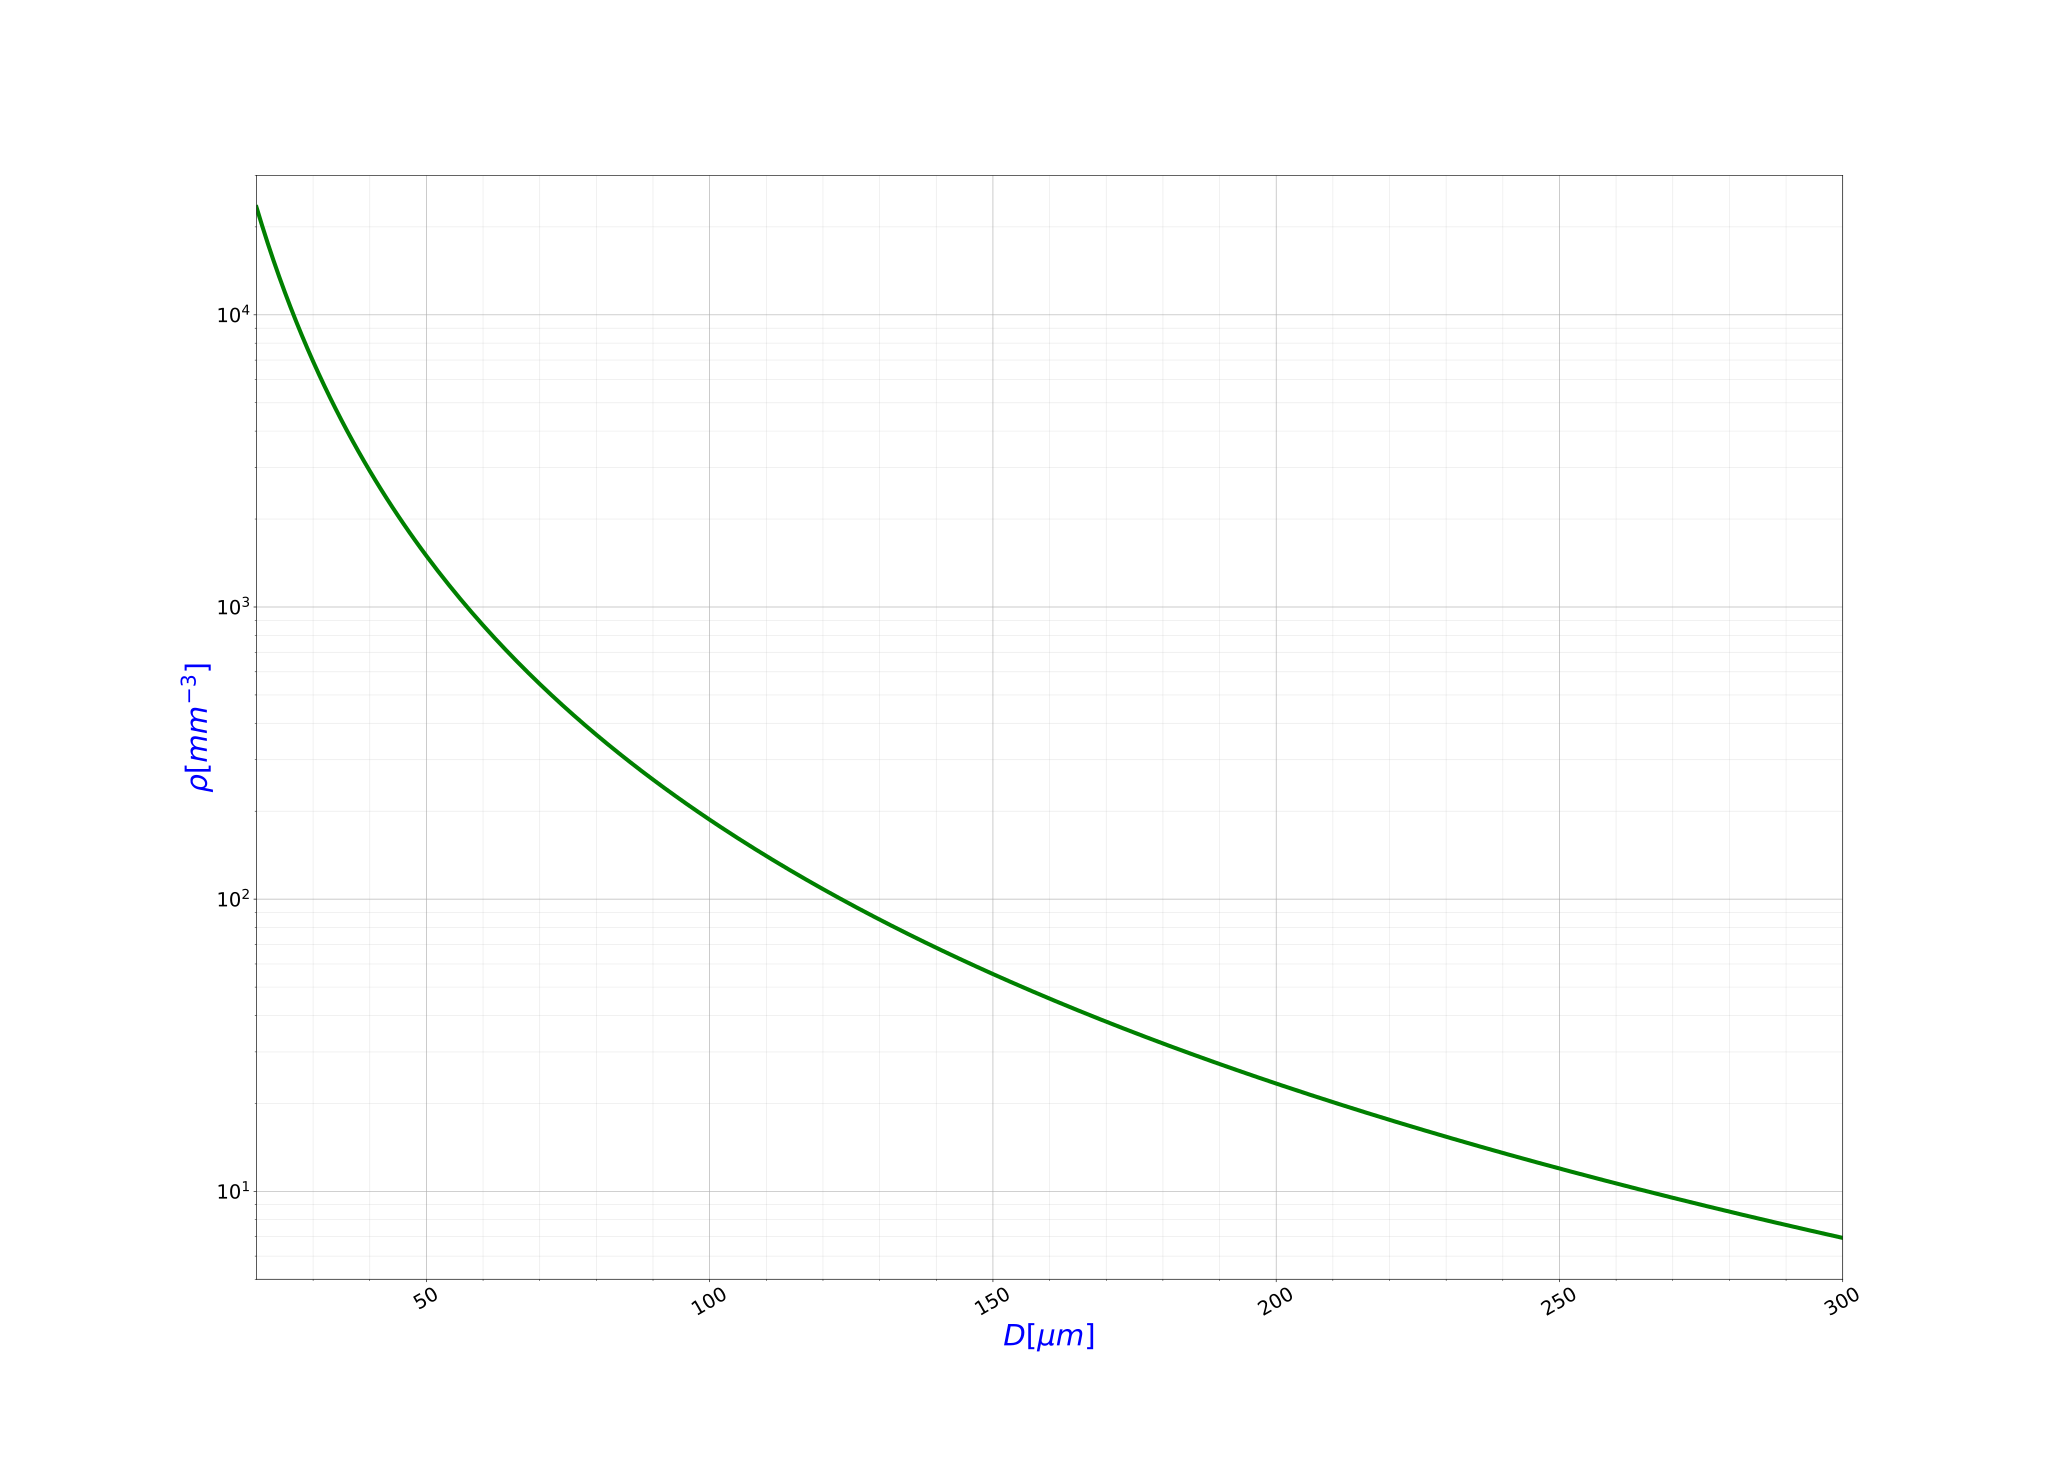
\includegraphics[width=\textwidth]{3_metodologia/curva_5_per_cent.png}
    \vspace{-15mm}
    \caption{\small Curva que relaciona el número de células $\rho$, con el diámetro de las \gotas\ $D$ a partir de un ajuste del tipo $y=ax^{-3}$ a los puntos (50,1496) (100,187). Esta curva permite el cálculo de las densidades de células en función del tamaño de las \gotas\ de modo que el número de encapsulados múltiples representa 5.15\% de los encapsulados únicos y el 4.89\% de los encapsulados totales. La distribución de encapsulados que se obtiene escogiendo $\rho$ de esta manera se ajusta es una distribución de Poisson con $\lambda=0.098$. La ecuación de la curva es la Ecuación~\ref{eq:rho}.}
    \label{fig:rho_d}
    \end{center}
\end{figure}

%Evidentemente, tamaño de las droples formadas en el sistema real no es uniforme y muestra una distribución de valores, a priori desconocida pero que se mantiene en un cierto rango. Cabe preguntarse como afecta la distribución de tamaño que adoptan las droplets a la proporción que se ha calculado entre las droplets sin encapsulado, las de encapsulado único y múltiple. En principio, podemos calcular la concentración que debería tener la muestra para aquellas que tienen un tamaño mayor y otro tamaños mas pequeños encontradas en la muestra y ver si hay alguna diferencia significativa entre las concentraciones calculadas. Si suponemos un tamaño de con valores observados máximos de y valores mínimos de vemos que estos valores son tan parecidos que están por debajo del error que comentemos a la hora de determinar la concentración de la muestra. Sin embargo resulta muy fácil hacer un programa que simule una situación en la que las droplets siguen una distribución conocida. Concretamente se ha hecho probado para el caso en el que las droplets muestran una distribución normal. En ningún sitio se ha probado en este trabajo que el tamaño responda a una distribución normal, 



\subsection{Concentración de cianobacterias en el cultivo.}

Para poder validar los resultados de nuestras simulaciones decidimos realizar encapsulaciones experimentales a distintas concentraciones celulares. Elegimos como modelo de estudio la cianobacteria unicelular Synechococcus elongatus PCC7942. Las razones para utilizar este microorganismo como modelo fueron las siguientes:

\begin{itemize}
    \item Tiene un tamaño celular de alrededor de 2 micras, lo que nos facilita el cumplimiento del axioma~1 en nuestro modelo computacional.
    \item Las cianobacterias contienen clorofila altamente fluorescente, lo que nos permitió determinar su presencia dentro de las gotas usando un microscopio de fluorescencia. Aunque las gotas son translúcidas, el coeficiente de difracción de la agarosa es muy parecido al del citoplasma celular. Esto dificulta mucho la detección de células dentro de las gotas en base a imágenes de contraste de fase. La autofluorescencia de las cianobacterias, que produce señales muy fuertes con exposiciones mínimas, nos permitió por tanto un sistema fiable de conteo. 
\end{itemize}

Las cianobacterias se crecieron en medio definido BG-11 , en condiciones de luz continua (500 mM de fotones), a 37~\celsius\ y con un 3\% de $\mathrm{CO}_{2}$ ambiental. En estas condiciones Synechococcus elongatus PCC7942 muestra un tiempo de generación de unas 4 horas. 

Para medir de manera exacta las concentraciones de células que introdujimos en cada experimento, la densidad de los cultivos se determinó mediante la cámara de Neubauer. La cámara de Neubauer es un instrumento que sirve para hacer recuentos de células en un volumen conocido, a partir de lo cual se puede determinar la densidad de células de la muestra analizada. Consta básicamente de un base de cristal sobre la que se ha grabado una rejilla de dimensiones conocidas y del tamaño similar a las células que se pretenden estudiar. Sobre esa base se coloca un cubreobjetos que al quedar apoyado sobre la base a una distancia conocida, delimita el volumen a estudiar.

Nosotros hemos utilizado para hacer los recuentos una cámara que consta de 9 cuadrados grandes de 1~mm de lado. Cada uno de estos, se encuentra a su vez subdividido en otros 16 medianos de 0.25~mm de lado. Los cuadrados medianos se vuelven a dividir, cada uno de ellos en 25 que conforman la rejilla de cuadros más pequeños, como puede verse en la Figura~\ref{fig:camara_neubauer}. 


\begin{figure}[H]
    \begin{center}
         \includegraphics[width=0.8\textwidth]{3_metodologia/plaq2.png}
         %\includesvg[angle=-90,height=15cm]{3_metodologia/curva_5_per_cent.svg}
        % \hspace{-17mm}{\includesvg[width=20cm]{3_metodologia/plaq2.png}}
    \caption{\small Representación de la base de la cámara Neubauer utilizada.(Imagen tomada de: \url{https://img.webme.com/pic/h/hematologiauis2013/plaq2.gif})}
    \label{fig:camara_neubauer}
    \end{center}
\end{figure}

La distancia a la que se encuentra el cubreobjetos de la base de la cámara es de 0.1~mm. La muestra a analizar se añade por uno de los lados de la cámara y entra por capilaridad hasta ocupar todo le volumen. Después se deja que las células se posen sobre el fondo.

Para hacer el recuento correctamente es importante utilizar la zona de la cuadrícula y el microscopio que mejor se ajusta al tamaño de las células. También es muy importante establecer un criterio para establecer qué células que se encuentran sobre alguno de los limites de la rejilla se van a contar y cuales no. Por ejemplo se puede establecer que solo se cuentan aquellas que se encuentran sobre la línea superior y lado derecho. Por último es necesario llevar un orden durante conteo para evitar dejar cuadros sin contar o contarlos dos veces. En muy fácil perderse cuando se realizan conteos mirando directamente con el microscopio, sobre todo si las células muestran pequeños desplazamientos.

Realizar recuentos mediante la cámara de Neubauer es tedioso. Para disponer de un sistema más rápido de estimación de las concentraciones de los cultivos, medimos también la densidad óptica a 750~\micrometro\ en un espectofotómetro Shimatzu UV-1580. A partir de estas medidas se elaboró una curva de calibración respecto a los resultados obtenidos en la cámara de Neubauer.

%Espectrofotómetro a 750 $\microm$

\subsection{Recuento de los encapsulados.}\label{sec:analisis_datos}

% descripción de la técnica
% microscopía confocal

Para comprobar la correlación entre las simulaciones y los resultados experimentales fue necesario desarrollar un sistema para evaluar la eficacia de los encapsulados. Para ello, como hemos apuntado antes, aprovechamos el hecho de la alta autofluorescencia de las cianobacterias dado su contenido en clorofila. De esta forma, utilizamos un microscopio de epifluorescencia Leica AXF500. Las gotas generadas por el chip se dispusieron en un portaobjetos y se analizaron con un objetivo de 10X aumentos. Tomamos imágenes en campo claro y de fluorescencia , usando para estas últimas un filtro para la fluorescencia en el canal del rojo Em 603-678 / Ex. 524-582. Dado que el tamaño de la cianobacteria es despreciable respecto al de la gota, escaneamos todo el volumen de esta realizando 30 Z-stacks. 

Los archivos obtenidos mediante esta técnica se componen de un conjunto de pares de imágenes tomadas a distintos planos; cada par tiene una imagen en el visible y otra tomada a la frecuencia emitida por la proteína fluorescente. En nuestro caso, al contener las cianobacterias clorofila, es esta la proteína que queremos encontrar para saber si el gota contiene célula en su interior o no. 

Los archivos que hemos utilizado para analizar las muestras, en nuestro caso tienen 30 planos de muestro que se toman desde la superficie de la muestra hasta poco más de los 100~\micrometro. El desplazamiento sobre el eje z (el eje vertical perpendicular a la muestra) viene determinado por el tamaño de las gotas de agarosa. El número de planos que debemos tomar lo determina el tamaño de las cianobactarias que estamos encapsulando. El tamaño típico de una cianobacteria es de 1-5~\micrometro. Lo ideal es que espaciado entre los muestreos sea inferior al tamaño del objeto que estamos buscando. Si suponemos un diametro de la gota de unos 100~\micrometro\ y tomamos 30~planos de muestreo el espaciado es de unos 3~\micrometro.

Para analizar las archivos se ha utilizado el programa Fiji Imagej. El programa cuenta con multitud de ajustes y opciones útiles que permiten poner de relieve los detalles que resultan de nuestro interés en las imágenes. Esto no supone, o no debe suponer de ningún modo la manipulación de la imagen para obtener los resultados deseados. Sin embargo es cierto que los ajustes están sujetos a cierto criterio subjetivo que dependerá de quién está realizando el análisis. Para realizar el análisis de la forma más objetiva posible, es importante establecer desde el inicio un criterio para tratar todas las imágenes de la misma forma y no modificar los archivos originales que se han realizado con el microscopio para que otro investigador pueda realizar un análisis propio, independiente del que nosotros hemos realizado.

En el caso del análisis de las imágenes a partir de las cuales se obtiene el recuento del número de encapsulados en las muestras analizadas, la manipulación que se ha realizado ha sido la proyección de la máxima intensidad alcanzada por las imágenes sobre un único plano. Las cianobacterias se han identificado como puntos rojos en la imagen de fluorescencia visibles sin necesidad de ningún otro tratamiento de la imagen. 

Para hacer el análisis se ha utilizado una herramienta de Fiji ImageJ que permite etiquetar objetos y facilita el recuento manual. Pertenecen al recuento solo las gotas de agarosa que se encontraban completamente dentro de la imagen y solo aquellas células que se encuentran dentro de esas gotas. De esta forma la muestra es algo más pequeña pero el análisis más conservador.

\section{Resultados.}\label{sec:4_resultados}

Los resultados aquí mostrados se engloban en dos bloques principales. Por un lado, incluimos un resumen de las condiciones óptimas de funcionamiento de la plataforma, en segundo lugar, mostramos la optimización de las concentraciones a encapsular. 

\subsection{Condiciones óptimas de funcionamiento.}\label{sec:4_resultados_puesta_a_punto}

En nuestro laboratorio disponemos de sistemas de bombas de jeringa y sistemas de control de presión de reservorios hidrostáticos. Durante las pruebas que hicimos para familiarizarnos con el funcionamiento del chip se usaron ambos sistemas y se compararon las ventajas y desventajas que ofrecían cada uno de ellos. Estas pruebas también mostraron que los flujos necesarios para formar gotas del tamaño y monodispersidad adecuados no tenían porque ser necesariamente grandes. Eran suficientes flujos de unos pocos microlitos por minuto en las dos fases para conseguir nuestro objetivo. Además, se concluyó que lo importante era la ratio entre los flujos, no tanto su magnitud.

A modo de resumen, las razones por las que se eligió el sistema de bombas de jeringa en vez del sistema de control de presión, fueron las siguientes:

\begin{itemize}

    \item Nos interesa un control del flujo, no un control de la presión. Controlar el flujo es trivial con una bomba de jeringa.
    
    \item Controlar de forma el flujo a partir ejerciendo una presión hidrostática requiere un ajuste continuo de la presión a partir de una medida continua del flujo. Debido a que la agarosa se solidifica a temperatura ambiente, no era aceptable arriesgarnos a obstruir el sensor de flujo haciendo pasar la agarosa por él, es decir, las bombas de jeringa no eran una opción para el circuito de agarosa.
    
    \item Controlar de forma manual la presión implica que en ocasiones los flujos aumenten de forma muy rápida e inesperada y perdamos la muestra en cuestión de apenas minutos.
    
    \item Las medidas con los sensores de flujo realizadas para la fase continua muestran que las bombas de jeringa son capaces de mantener flujos bajos de una forma más regular que el sistema de presión.
    
    \item Purgar los tubos resultaba una tarea engorrosa debido a las diferencias de nivel en la plataforma. Mejorar este aspecto la era uno de los objetivos cuando se diseño la platina del microscopio, sin embargo el sistema de presión esta diseñado para trabajar con tubos eppendorf en posición vertical y esto no se podía cambiar tan fácilmente. La altura de estos tubos es de 3~cm y esto provocaba el retorno del fluido al reservorio hidrostático al detener la presión.
    
\end{itemize}


Los flujos finales para hacer los encapsulados fueron 2.25~\microlitrosporminuto\ para la fase dispersa (agarosa) y 6~\microlitro\ para la fase continua (aceite). Las pruebas que se hicieron previas a los encapsulados mostraron que estos flujos se corresponden con tamaños de gotas de agarosa que rondan los 125~\micrometro. La estimación del tamaño de las gotas se hizo a partir del análisis de las imágenes de las gotas tomadas por una cámara de alta velocidad en el orificio del salida del chip. Esta estimación, sirvió para fijar el diámetro de la gota antes de empezar los experimentos de encapsulado de forma que pudimos estimar la concentración de células que debe tener la muestra a encapsular.


\subsection{Optimización de las concentraciones a encapsular.}

\subsubsection{Ajuste lineal entre los recuentos cámara de Neubauer y la densidad óptica.}

Para establecer la relación lineal entre los recuentos de células y la densidad óptica se hicieron las medidas que se muestran en la Tabla~\ref{tab:resultados_neubauer}.

\begin{spacing}{1}

\begin{table}[H]
\renewcommand\tablename{Tabla}
\renewcommand{\arraystretch}{1.5}
\centering
    
    \setlength{\extrarowheight}{-2pt}
    \begin{tabular}{ R{1.2cm} C{0.8cm} C{1.1cm} C{0.4cm} C{0.4cm} C{0.4cm} C{0.4cm} C{0.4cm} C{0.4cm} C{0.4cm} C{0.4cm} C{0.4cm} C{0.4cm} C{0.4cm} C{0.4cm} C{0.4cm} C{0.4cm} C{0.4cm} }
        \hline
        OD\small{$750$}	& Vol & D & a & b & c & d & e & f & g & h & i & j & k & l & m & n & o \\
        %\cline{1-3}
        \hline
        \hline
        

0,071	&	250	&	1	&	29	&	69	&	51	&	38	&	40	&	42	&	28	&	31	&	34	&	36	&	34	&	33	&	52	&	56	&	69	\\
0,0149	&	250	&	10	&	5	&	20	&	18	&	40	&	12	&	17	&	10	&	19	&	31	&	12	&	14	&	12	&	4	&	10	&	14	\\
0,0149	&	250	&	10	&	4	&	3	&	4	&	5	&	0	&	7	&	3	&	4	&	2	&	5	&	6	&	3	&	3	&	5	&	5	\\
0,0149	&	250	&	10	&	9	&	7	&	5	&	4	&	4	&	3	&	6	&	7	&	5	&	2	&	3	&	7	&	2	&	5	&	2	\\
0,1748	&	500	&	1	&	75	&	68	&	60	&	63	&	59	&	57	&	49	&	50	&	62	&	58	&	61	&	60	&	71	&	52	&	63	\\
0,1748	&	500	&	1	&	59	&	57	&	67	&	90	&	58	&	63	&	85	&	47	&	58	&	86	&	79	&	50	&	59	&	61	&	83	\\
0,028	&	250	&	10	&	50	&	38	&	69	&	67	&	25	&	47	&	32	&	65	&	39	&	42	&	25	&	29	&	17	&	17	&	25	\\
0,0063	&	250	&	100	&	14	&	30	&	83	&	44	&	24	&	8	&	29	&	37	&	41	&	-	&	50	&	24	&	23	&	34	&	64	\\
0,0063	&	250	&	100	&	6	&	8	&	5	&	19	&	0	&	4	&	4	&	4	&	1	&	1	&	0	&	3	&	2	&	2	&	1	\\
0,0447	&	1000	&	10	&	12	&	11	&	7	&	6	&	12	&	12	&	8	&	12	&	9	&	9	&	7	&	4	&	6	&	9	&	6	\\
0,0115	&	1000	&	100	&	2	&	3	&	2	&	3	&	3	&	5	&	4	&	1	&	6	&	4	&	3	&	7	&	3	&	1	&	3	\\
        
        \hline
    \end{tabular}

    \caption{\small Resultados de los recuentos de células realizados con la cámara de Neubauer. Cada fila contiene los datos relativos a una muestra estudiada. La primera columna empezando por la izquierda, contiene las medidas de la densidad óptica (OD) de cada una de las muestras. La segunda columna llamada  Vol, contiene el valor del volumen por el que hay que multiplicar el número de recuentos  para obtener en número de células por $\mathrm{mm^{3}}$. La tercera la dilución de la muestra y el resto de columnas contiene los valores de cada uno de los recuentos realizados.}
    \label{tab:resultados_neubauer}
    
\end{table}

\end{spacing}

Estas medidas se realizaron en el transcurso de varios días y a partir de varios cultivos diferentes.
A partir de estos datos se obtienen los valores de la Tabla~\ref{tab:analisis_neubauer}.

% \begin{table}[H]
% \renewcommand\tablename{Tabla}
% \renewcommand{\arraystretch}{1.5}
% \centering
    
%     \setlength{\extrarowheight}{-2pt}
%     \begin{tabular}{ C{2cm} C{2cm}  C{2cm} C{2cm} C{2cm} C{2cm} }
%         \hline
%         OD\small{$750$}	& $\bar{x}$ & $\sigma$ & Vol & N/cell &  $\sigma$\\
%         %\cline{1-3}
%         \hline
%         \hline
% % 0.071	&	42.8	&	250	    &	10700	&	3276	\\
% % 0.0149	&	15.9	&	250	    &	3967	&	2258	\\
% % 0.0149	&	3.9	    &	250	    &	983	    &	413	    \\
% % 0.0149	&	4.7	    &	250	    &	1183	&	520	    \\
% % 0.1748	&	60.5	&	500	    &	30267	&	3483    \\	
% % 0.1748	&	66.8	&	500	    &	33400	&	6763	\\
% % 0.028	&	39.1	&	250	    &	9783	&	4213	\\
% % 0.0063	&	36.1	&	250	    &	9017	&	4768	\\
% % 0.0063	&	4.0	    &	250	    &	1000	&	1144	\\
% % 0.0447	&	8.7	    &	1000	&	8667	&	2573	\\
% % 0.0115	&	3.3	    &	1000	&	3333	&	1619	\\



% 0.071	&	43	&	13	&	250	    &	11000	&	3000	\\
% 0.0149	&	16	&	9	&	250	    &	4000	&	2000	\\
% 0.0149	&	4	&	2	&	250	    &	1000	&	400	    \\
% 0.0149	&	5	&	2	&	250	    &	1000	&	500	    \\
% 0.1748	&	60	&	7	&	500	    &	30000	&	3000    \\	
% 0.1748	&	67	&	13	&	500	    &	33000	&	7000	\\
% 0.028	&	40	&	16	&	250	    &	10000	&	4000	\\
% 0.0063	&	36	&	19	&	250	    &	9000	&	5000	\\
% 0.0063	&	4	&	5	&	250	    &	1000	&	1000	\\
% 0.0447	&	9	&	3	&	1000	&	9000	&	3000	\\
% 0.0115	&	3	&	2	&	1000	&	3000	&	2000	\\


% 0.071	&	43	&	13	&	250	    &	11000	&	3000	\\
% 0.0149	&	16	&	9	&	250	    &	4000	&	2000	\\
% 0.0149	&	4	&	2	&	250	    &	1000	&	400	    \\
% 0.0149	&	5	&	2	&	250	    &	1000	&	500	    \\
% 0.1748	&	60	&	7	&	500	    &	30000	&	3000    \\	
% 0.1748	&	67	&	13	&	500	    &	33000	&	7000	\\
% 0.028	&	40	&	16	&	250	    &	10000	&	4000	\\
% 0.0063	&	36	&	19	&	250	    &	9000	&	5000	\\
% 0.0063	&	4	&	5	&	250	    &	1000	&	1000	\\
% 0.0447	&	9	&	3	&	1000	&	9000	&	3000	\\
% 0.0115	&	3	&	2	&	1000	&	3000	&	2000	\\

        
%         \hline
%     \end{tabular}

%     \caption{\small Datos obtenidos a partir del análisis de los datos contenidos en la Tabla~\ref{tab:resultados_neubauer}. Se vuelve a mostrar los valores de la densidad óptica y a partir de los recuentos de cada fila en la tabla anterior se calculan los valores medios, el número de células por y la desviación estándar. Los números que aparecen en la tabla se han redondeado para dejar una cifra entera en las columnas de los valores medios de los recuentos y su desviación estándar. En el caso de la densidad de células y su desviación estándar, el redondeo se ha realizado de modo que quede una cifra significativa.}
%     \label{tab:analisis_neubauer}
    
% \end{table}

\begin{spacing}{1}

\begin{table}[H]
\renewcommand\tablename{Tabla}
\renewcommand{\arraystretch}{1.5}
\centering
    
    \setlength{\extrarowheight}{-2pt}
    \begin{tabular}{ C{2cm} C{2cm}  C{2cm} C{2cm} C{2cm} C{2cm} }
        \hline
        OD\small{$750$}	& $\bar{x}$ & $\sigma$ & Vol & N$\times {10}^{3} $ &  ${\sigma}_{N} \times {10}^{3}$\\
        %\cline{1-3}
        \hline
        \hline

0.071	&	43	&	13	&	250	    &	11	&	3	\\
0.0149	&	16	&	9	&	250	    &	4	&	2	\\
0.0149	&	4	&	2	&	250	    &	1	&	0.4	    \\
0.0149	&	5	&	2	&	250	    &	1	&	0.5	    \\
0.1748	&	60	&	7	&	500	    &	30	&	3    \\	
0.1748	&	67	&	13	&	500	    &	33	&	7	\\
0.028	&	40	&	16	&	250	    &	10	&	4	\\
0.0063	&	36	&	19	&	250	    &	9	&	5	\\
0.0063	&	4	&	5	&	250	    &	1	&	1	\\
0.0447	&	9	&	3	&	1000	&	9	&	3	\\
0.0115	&	3	&	2	&	1000	&	3	&	2	\\

        \hline
    \end{tabular}

    \caption{\small Datos obtenidos a partir del análisis de los datos de la Tabla~\ref{tab:resultados_neubauer}. La columna $\bar{x}$ contiene los valores medios de los recuentos y $\sigma$ la desviación estándar de los mismos. De la misma forma N contiene los valores del número de células por $\mathrm{mm^{3}}$ contenido en las muestras y ${\sigma}_{\mathrm{N}}$ es desviación estándar de esos valores. Los valores se han redondeado para dejar una cifra entera en las columnas de los valores medios de los recuentos y su desviación estándar. En el caso de la N y su desviación estándar, el redondeo se ha realizado de modo que quede una cifra significativa.}
    \label{tab:analisis_neubauer}
    
\end{table}

\end{spacing}

A partir de la representación de los valores de la Figura~\ref{fig:recuentos_camara_neubauer}. La recta representada es un ajuste lineal a la recta $y=ax$.
%Coeficiente de determinacion
%Coefficient of determination

\begin{figure}[H]
    \begin{center}
        \includegraphics[width=0.8\textwidth]{4_resultados/ajuste_rho_cultivo.png}
         %\includesvg[angle=-90,height=15cm]{3_metodologia/curva_5_per_cent.svg}
        % \hspace{-17mm}{\includesvg[width=20cm]{3_metodologia/cama}}
    \caption{\small Ajuste lineal entre los recuentos cámara de Neubauer y la densidad óptica, a partir del cual se hacen las estimaciones del número de células en el cultivo. Los valores numéricos de los puntos utilizados para representar están contenidos en la Tabla~\ref{tab:analisis_neubauer}. Las barras de error se han generado a partir de los valores de la desviación estándar de los recuentos. La ecuación de la recta de ajuste es $\rho=182533\times \mathrm{OD}$. Para realizar los cálculos resulta más cómodo trabajar en ml. En ese caso la pendiente queda multiplicada por 1000.}
    \label{fig:recuentos_camara_neubauer}
    
    \end{center}
\end{figure}

El valor de la pendiente de la recta de ajuste de la figura anterior, se utilizará para calcular los valores de la concentración de células en el cultivo en la Sección~\ref{sec:resultados:encapsulados}.

\subsubsection{Encapsulados.}\label{sec:resultados:encapsulados}

Para probar que efectivamente podíamos encapsular cianobacterias con nuestro dispositivo experimental, utilizamos dos muestras con dos concentraciones diferentes. La muestra 1x tiene una concentración óptima de células para que el número de encapsulados múltiples represente el 5\% de los encapsulados totales, suponiendo un diámetro de la gota de 125~\micrometro. La muestra 10x tiene una concentración de células 10 veces superior a la muestra anterior. En ambos casos se utilizó el chip con dos entradas (ver Figura~\ref{fig:chips}) y la muestra a encapsular ya tiene células diluidas en la agarosa. Los flujos fueron $2.25~\mathrm{\mu l}$ para la fase dispersa (agarosa) y $6~\mathrm{\mu l}$ para la fase continua (aceite) que se corresponden para un diámetro de $\sim125~\mathrm{\mu m}$ como ya se ha mencionado en la Sección~\ref{sec:4_resultados_puesta_a_punto}. La temperatura a la que se mantuvo la agarosa hasta llegar al chip fue de 43~\celsius.

Ambas muestras se prepararon a partir del mismo cultivo, el mismo día. La concentración de células en la muestra original se obtuvo a partir una medida con el espectrofotómetro de 0.4832 a $750~\mathrm{\mu m}$. Teniendo en cuenta el ajuste de la Figura~\ref{fig:recuentos_camara_neubauer} se obtiene un valor de $\sim 82\cdot{10}^{6}$ cel/ml. Las dos muestras que se prepararon tenían un volumen de $\sim250~\mathrm{\mu l}$ con una concentración de agarosa de $\sim 1 \%$.

\subsubsection{Muestra 1x.}\label{muestra1x}

Supusimos, partiendo de experimentos previos que el diámetro de las gotas que se iban a formar rondaría los 125~\micrometro. Partiendo de este dato y la curva de ajuste mostrada en la Figura \ref{fig:rho_d} se estimó que la concentración de células necesaria para la distribución de encapsulados que nosotros estábamos buscando era de $\sim98\cdot{10}^{3}\;\mathrm{cel\;mm^{-3}}$ que corresponde a $1.2~\mathrm{\mu l}$ de la muestra original. Debido a que se trata de una cantidad bastante pequeña se preparó una dilución -2 a partir de la muestra original y de esta se cogieron 30~\microlitro\ que se mezclaron con 220~\microlitro\ de una dilución de agarosa al 1\%. El tiempo durante el cual se estuvieron formando \gotas\ esta entorno a los 15~min.

En la Figura~\ref{fig:imagenes_1x} se muestran dos imágenes que pretenden ser representativas de la muestra de \gotas\ obtenidas. En estas imágenes obtenidas mediante epifluorescencia, muestran una serie de puntos rojos que efectivamente se han producido los encapsulados. Lo que buscamos ahora es estudiar en que proporción se han producido los encapsulados, para saber si la muestra de gotas es la adecuada para hacer análisis genómico de las células que contienen. Para ello se va a realizar un recuento del número de gotas completas por imagen, y de estas cuantas tienen encapsulados únicos y múltiples. Los resultados obtenidos se muestran en la Tabla~\ref{tab:resultados_1x}.

\begin{figure}[H]
  \begin{center} 
  
    \subfloat[]{
     \label{subfig:1x_11}
      \includegraphics[width=0.4\textwidth]{4_resultados/1x_imag5_bar_scale.png}}
    \subfloat[]{
     \label{subfig:1x_12}
      \includegraphics[width=0.4\textwidth]{4_resultados/1x_imag12_scale_bar.png}}
      
    % \subfloat[]{
    %  \label{subfig:ajuste_c}
    %   \includegraphics[width=0.5\textwidth]{4_resultados/1x_img21_recuentos.png}} 
    % \subfloat[]{
    %  \label{subfig:ajuste_d}
    %   \includegraphics[width=0.5\textwidth]{4_resultados/1x_img21_recuentos.png}} 

  \end{center}
  \vspace{-5mm}    
  \caption{\small Imágenes representativas de la muestra 1x. Las imágenes de la Figura~\ref{subfig:1x_11} y \ref{subfig:1x_12} representadas se corresponden con las imágenes llamadas 11 y 12 del a Tabla~\ref{tab:resultados_1x}. Los números que aparecen sobre las gotas hacen referencia al conteo manual que se ha realizado. El 1 indica que la gota se ha tenido en cuenta para hacer el recuento del número de gotas en la imagen. Los números mayores que 1 quieren decir que las gotas cuentan con encapsulados. El número de encapsulados es igual a número asignado menos 1. Los criterios que se han utilizado para realizar los recuentos se explican con detalle en la Sección~\ref{sec:analisis_datos}. La escala que aparece en la esquina inferior derecha representa una longitud de 100 micras en la imagen. }
  \label{fig:imagenes_1x}
\end{figure}



\begin{spacing}{1}

\begin{table}[H]
\renewcommand\tablename{Tabla}
\renewcommand{\arraystretch}{1.5}
\centering
    
    \setlength{\extrarowheight}{-2pt}
    \begin{tabular}{ C{2cm} C{2cm} C{2cm} C{2cm} C{2cm} C{2cm} }
        \hline
        Imagen	& N gotas	& 0 encap & 1 encap & 2 encap & 3 encap\\
        %\cline{1-3}
        \hline
        \hline
        
1	&	38	&	36	&	2	&	0	&	0	\\
2	&	26	&	21	&	4	&	1	&	0	\\
8	&	41	&	36	&	4	&	1	&	0	\\
9	&	46	&	40	&	6	&	0	&	0	\\
11	&	46	&	42	&	4	&	0	&	0	\\
12	&	45	&	40	&	5	&	0	&	0	\\
17	&	33	&	27	&	5	&	1	&	0	\\
18	&	9	&	8	&	1	&	0	&	0	\\
20	&	28	&	24	&	3	&	1	&	0	\\
21	&	32	&	25	&	4	&	2	&	1	\\
    
        \hline
        $\sum{x_i}$	& 344 	& 299 	& 38 	& 6 	& 1 \\
        \small{$\% \mathrm{(N\;gotas )}$}	& 100 & 87 & 11 & 2 & 0 \\
        \hline
    \end{tabular}

    \caption{\small Recuentos del número de encapsulados que se han producido en cada una de las imágenes para la muestra~1. Los valores de la columna imagen permiten identificar la imagen a partir de la cual se ha hecho cada uno de los recuentos. Por ejemplo, las imágenes 11 y 12 son las que aparecen en la Figura~\ref{subfig:1x_11} y Figura~\ref{subfig:1x_12} respectivamente. La antepenúltima fila representa el sumatorio de cada una de las columnas que se encuentran inmediatamente por encima y la última el porcentaje del sumatorio relativo a total de \gotas.}
    \label{tab:resultados_1x}
    
\end{table}
\end{spacing}

Las imágenes también nos permiten medir el tamaño de las gotas con las herramientas proporcionadas por Fiji.
Tras realizar la medida de 100 \gotas\ sobre las imágenes y suponiendo que la distribución de diámetros sigue una distribución normal tenemos que el diámetro de las \gotas\ es $102\pm16\mathrm{\mu m}$ cuando lo que esperábamos era un diámetro de la \gota\ de $\sim125\mathrm{\mu m}$.

Por tanto, llegados a este punto tenemos el recuento de los encapsulados que se han producido, una medida del tamaño de las gotas y un cálculo previo de la densidad de células de la muestra calculada a partir una medida de la densidad óptica del cultivo. También sabemos que independientemente de la concentración de células de la muestra, la proporción entre los encapsulados debe ajustarse a una distribución de Poisson y que esa distribución se caracteriza el parámetro $\lambda$. 
Lo que se hace a continuación obtener el parámetro $\lambda$ de la distribución de Poisson que mejor se ajusta a las proporciones observadas, mediante un ajuste por mínimos cuadrados. Después se obtiene la concentración de células de la muestra partiendo del parámetro $\lambda$ anterior y se compara con el $\lambda$ obtenido suponiendo la que concentración de células en la muestra era la que habíamos calculado. Los resultados de esta comparación se muestran en la Tabla~\ref{tab:comparacion_porcentajes_1x}

% Lo que se hace hace a continuación es comparar el paramentro landa de la distribución de poisson ajustada a la proporion de encapsulados observados con la distribución esperada suponiendo la concentración de celulas en la muestra y se obtiene la concentración de celulas en la muestra suponiendo un parametro landa igual al del ajuste de encapsulados observados. Los resultados de esta comparación se muestran en la Tabla~\ref{tab:comparacion_porcentajes_1x}.

\begin{spacing}{1}
\begin{table}[H]
\renewcommand\tablename{Tabla}
\renewcommand{\arraystretch}{1.5}
\centering
    
    \setlength{\extrarowheight}{-2pt}
    \begin{tabular}{C{1cm} C{1.5cm} C{2.2cm} C{1.5cm} C{1.5cm} C{1.5cm} C{1.5cm}}
        \hline
         & $\lambda$ & \small{$\rho\:(\mathrm{cel\;{mm}^{-3}})$} & 0 encap & 1 encap & 2 encap & 3 encap\\
        \hline
        \hline
        
        $r$ & 0.1286 & x & 87 & 11 & 2 & 0 \\
        $e$ & 0.0544 & 98 & 95 & 5 & 0 & 0 \\
        $a$ & 0.1291 & 233 & 88 & 11 & 1 & 0 \\
        
        \hline
    \end{tabular}

    \caption{\small Comparación los valores de $\lambda$, densidad de células en la muestra y porcentajes de los recuentos de encapsulados obtenidos a de tres formas diferentes. Las letras que aparecen en la primera columna indican si los valores de la fila pertenecen a los valores obtenidos a partir de los recuentos hechos con las imágenes $r$, los valores esperados suponiendo correcta la concentración de células de 98~$\mathrm{cel\;{mm}^{-3}}$ llamada $e$ (el Apéndice~\ref{apendice:salida} muestra las salida relativa a este cálculo) y por último los valores proporcionados por una simulación con la concentración de células de modo que el valor de $\lambda$ es el mismo al valor de la fila $a$. $\lambda$ es un valor que caracteriza a la distribución de Poisson. El valor de $\lambda$ de la fila $r$ se obtiene a partir de un ajuste por mínimos cuadrados de una distribución de Poisson multiplicada por un factor de escala a los recuentos totales del número de \gotas\ de la Tabla~\ref{tab:resultados_1x}. Todas las simulaciones parten de los valores volumen de la muestra 250~\milimetrocubico\ diámetro de la \gota\ $102\pm16$~\micrometro\ y número de simulaciones 4.}
    \label{tab:comparacion_porcentajes_1x}
    
\end{table}

\end{spacing}

Este resultado indica que la distribución de Poisson que mejor se ajusta a las proporciones observadas en la muestra es aquella con $\lambda=$0.1286 que se corresponde con una densidad de células de $\sim$233~$\mathrm{cel\;{mm}^{-3}}$ lo que supone un valor 2.4 veces superior a la concentración de células que habíamos calculado inicialmente. 

\subsubsection{Muestra 10x.}\label{muestra10x}

En el caso de la segunda muestra, el procedimiento fue el mismo que en el caso anterior. Se supuso que el tamaño de la gota seria el  mismo, 125~\micrometro, pero este caso se cogieron 30~\micrometro\ de la dilución -1 para tener una concentración de células 10 veces mayor que la muestra anterior.

De nuevo se estudian 10 imágenes y se hace un recuento del número de encapsulados que se encuentran en las \gotas\ que están completas. La Figura~\ref{fig:imagenes_10x} muestra dos de las imágenes utilizadas para hacer el recuento de las gotas y los resultados completos de este recuento se recogen en la Tabla~\ref{tab:resultados_10x}. El diámetro de las gotas en este caso es de $124\pm6$ lo cual se aproxima bastante al valor esperado. La comparación entre la distribución de Poisson que mejor se ajusta a los valores observados, los valores esperados y la concentración de células de la muestra obtenida a partir de los recuentos se recoge en la Tabla~\ref{tab:comparacion_porcentajes_10x}.

\begin{spacing}{1}
\begin{table}[H]
\renewcommand\tablename{Tabla}
\renewcommand{\arraystretch}{1.5}
\centering
    
    \setlength{\extrarowheight}{-2pt}
    \begin{tabular}{ C{1cm} C{1.5cm} C{2.2cm} C{1.5cm} C{1.5cm} C{1.5cm} C{1.5cm} C{1.5cm} C{1.5cm} }
        \hline
         & $\lambda$ & \small{$\rho\:(\mathrm{cel\;{mm}^{-3}})$} & 0 encap & 1 encap & 2 encap & 3 encap & 4 encap & 5 encap \\
        \hline
        \hline
        $r$ & 0.961 & x & 39 & 29 & 21 & 7 & 3 & 0 \\
        $e$ & 0.976 & 980 & 38 & 37 & 18 & 6 & 1 & 0 \\
        $a$ & 0.966 & 930 & 40 & 36 & 17 & 5 & 1 & 0 \\
        \hline
    \end{tabular}

    \caption{\small Comparación los valores de $\lambda$, densidad de células en la muestra y porcentajes de los recuentos de encapsulados obtenidos a de tres formas diferentes. Las letras que aparecen en la primera columna indican si los valores de la fila pertenecen a los valores obtenidos a partir de los recuentos hechos con las imágenes $r$, los valores esperados suponiendo correcta la concentración de células de 980 cel/mm3 $e$ y por ultimo los valores proporcionados por una simulación con la concentración de células de modo que el valor de $\lambda$ es el mismo al valor de la fila $a$. $\lambda$ es un valor que caracteriza a la distribución de Poisson. El valor de $\lambda$ de la fila $r$ se obtiene a partir de un ajuste por mínimos cuadrados de una distribución de Poisson multiplicada por un factor de escala a los recuentos totales del número de \gotas\ de la Tabla~\ref{tab:resultados_10x}. Todas las simulaciones parten de los valores volumen de la muestra 250~\milimetrocubico\ diámetro de la \gota\ $124\pm6$~\micrometro\ y número de simulaciones 4. }
    \label{tab:comparacion_porcentajes_10x}
    
\end{table}
\end{spacing}

En este caso la distribución de Poisson que mejor se ajusta a las proporciones observadas en la muestra es aquella con $\lambda$=0.961 que se corresponde con una densidad de células de $\sim930\;\mathrm{cel\;mm^{-3}}$ . En este caso la diferencia entre la concentración de células en la muestra que habíamos estimado previa al experimento y la calculada a partir de los encapsulados que se han producido es algo mayor a 5\%.

% \newpage

\begin{figure}[H]
  \begin{center} 
  
    \subfloat[]{
     \label{subfig:10x_a}
      \includegraphics[width=0.45\textwidth]{4_resultados/10x_imag4_b_escala4.png}}
    \subfloat[]{
     \label{subfig:10x_b}
      \includegraphics[width=0.45\textwidth]{4_resultados/10x_imag7_b_escala.png}}

  \end{center}
  \vspace{-5mm}    
  \caption{\small Imágenes representativas de la muestra 10x. Las imágenes de la Figura~\ref{subfig:10x_a} y \ref{subfig:10x_b} representadas se corresponden con las imágenes llamadas 2 y 7 del a Tabla~\ref{tab:resultados_10x}. De nuevo, los números que aparecen sobre las gotas hacen referencia a la conteo manual que se ha realizado. En 1 indica que la gota se ha tenido en cuenta para hacer el recuento del número de gotas en la imagen. Los números mayores que 1 quieren decir que las gotas cuentan con encapsulados. El número de encapsulados es igual a número asignado menos 1. Los criterios que se han utilizado para realizar los recuentos son los mismos que en el caso de la Figura~\ref{fig:imagenes_1x}. La escala que aparece en la esquina inferior derecha representa una longitud de 100 micras. }
  \label{fig:imagenes_10x}
\end{figure}

\begin{spacing}{1}
\begin{table}[H]
\renewcommand\tablename{Tabla}
\renewcommand{\arraystretch}{1.5}
\centering
    
    \setlength{\extrarowheight}{-2pt}
    \begin{tabular}{ C{2cm} C{2cm} C{2cm} C{2cm} C{2cm} C{2cm} C{2cm} C{2cm} }
        \hline
        Imagen	& N gotas	& 0 encap & 1 encap & 2 encap & 3 encap & 4 encap \\
        %\cline{1-3}
        \hline
        \hline
        
1	&	29	&	14	&	8	&	3	&	3	&	1	\\
2	&	28	&	14	&	8	&	4	&	2	&	0	\\
3	&	31	&	13	&	11	&	6	&	1	&	0	\\
4	&	29	&	12	&	10	&	4	&	3	&	0	\\
5	&	29	&	8	&	7	&	10	&	4	&	0	\\
6	&	27	&	7	&	11	&	5	&	1	&	3	\\
7	&	29	&	13	&	7	&	7	&	1	&	1	\\
8	&	30	&	14	&	7	&	7	&	1	&	1	\\
9	&	28	&	10	&	8	&	8	&	2	&	0	\\
10	&	28	&	8	&	7	&	8	&	3	&	2	\\

        \hline
        $\sum{x_i}$	& 288 & 113 & 84 & 62 & 21 & 8 \\
        \small{$\% \mathrm{(N\;gotas)}$}	& 100 & 39 & 29 & 21 & 7 & 3 \\
        \hline
    \end{tabular}

    \caption{\small Recuentos del número de encapsulados que se han producido en cada una de las imágenes para la muestra 10x. Los valores de la columna imagen identifican la imagen a partir de la cual se ha hecho cada uno de los recuentos. La antepenúltima fila representa el sumatorio de cada una de las columnas que se encuentran inmediatamente por encima y la última el porcentaje del sumatorio relativo a total de \gotas.}
    \label{tab:resultados_10x}
    
\end{table}
\end{spacing}

% Random seed =  7 
% $\rho$ =  980.0 1 / mm3 
% Volumen de la muestra:  250.0 mm3 
% Diámetro droplet:  124.0 micron 
% Flujo fase dispersa:  3.0 mm3 / min 
% Número de simulaciones:  4 

% Desviación estándar relativo al tamaño de la droplet expresado como tanto por 1: 0.05 

% El número de encapsulados múltiples representa el  69.936414265416 de los encapsulados únicos.

% El número de encapsulados múltiples representa el 41.154460371386605 de los encapsulados totales. Nuestro objetivo es que se encuentre en el 5\%.

% Porcentaje que representa cada conjunto de droplets con distinto número de encapsulados respecto del total de la muestra:

%  [37.67735417323904, 36.67662339218184, 17.997879536932395, 
%  5.858428141859378, 1.4495820970621005, 0.2853240794355016, 
%  0.05151407452369447, 0.006289509098823163,0.0012978352108682718, 
%  0.00019966695551819564]
 
 
 
% Lo que se parece:
 
 
 
 
%  Random seed =  7 
% ρ =  930.0 1 / mm3 
% Vol_muestra:  250.0 mm3 
% Diametro droplet:  124.0 micron 
% Flujo fase dispersa:  3.0 mm3 / min 
% Número de simulaciones:  4 
% Desviación estandar relativo al tamaño de la droplet expresado como tanto por 1: 0.05 

% El número de encapsulados multiples representa el  65.0325772431116 % de los encapsulados únicos.

% El número de encapsulados multiples representa el 39.40590296139609 % de los encapsulados totales. Nuestro objetivo es que se encuentre en el 5%.

% Porcentaje que representa cada conjunto de droplets con distinto número de encapsulados respecto del total de la muestra:
%  [39.59241778075934, 36.60403389397352, 17.014371396169757, 5.276566518120976, 1.24586707556663, 0.21942434552046897, 0.040929927963326784, 0.006988036481543597, 0.00039931637037391983, 9.982909259347996e-05]

\section{Discusión.}\label{sec:5_discusion}

%En la discusión se resumen, interpretan y extrapolan los resultados, se analizan sus implicaciones y limitaciones, y se confrontan con las hipótesis planteadas, considerando cómo ha sido la perspectiva de otros autores.

%En otras palabras, se hace énfasis en aspectos resumidos y escuetos del estudio, planteamiento de propuestas de investigaciones futuras, comparación con otros estudios, presentación de las limitaciones del estudio y de la posible generalización de los resultados, de otros hallazgos no previstos y de la interpretación de los resultados por el investigador, entre otros aspectos. Este artículo se centrará en desarrollar específicamente este tópico.

Los sistemas de inyección de jeringa han mostrado ser un método más práctico para nuestro propósito que los sistemas de control de presión. Los flujos que nosotros hemos encontrado como óptimos en la generación de las gotas son parecidos a los que hacen referencia otros autores como \cite{article:hirose}, que utilizan un chip con una simetría y tamaño de canal al chip de la Figura~\ref{subfig:chip3}. 

Se ha mostrado que somos capaces de obtener una muestra de gotas de agarosa con una concentración del 1\% con un diámetro muy próximo a las 125 micras y una desviación estándar que ronda el 5\% (ver Sección~\ref{muestra10x}). Los autores \cite{article:hirose} aseguran haber conseguido gotas de agrosa a una concentración del 3\% y un diámetro de 50~micras con una desviación estándar entorno al 1\%. En el caso de \cite{article:haakan} citan a autores que también consiguen desviaciones en el tamaño de entre el 1\% y el 3\%, pero no nos informan sobre la composición de la fase dispersa; en \cite{article:ralf} se habla de desviaciones de entrono al 2\% pero de nuevo, tampoco nos indican la composición de la fase dispersa. Es necesario un estudio minucioso de la metodología para identificar qué podemos mejorar para conseguir una mejor monodispersidad de las gotas. 

En numerosos artículos señalan que la distribución de encapsulados debe seguir una distribución de Poisson, partiendo de una muestra con las características descritas en la Sección~\ref{subsec:concentracion_celulas}. En el artículo de \cite{article:haakan} nos indica que el promedio células por gota (el valor de $\lambda$ en la distribución de Poisson) debe situarse entre 0.1 y el 1. En \cite{article:sarah} nos indican que, dependiendo de la aplicación, lo que se busca típicamente es una distribución con $\lambda=0.1$, $\lambda=0.3$ o $\lambda=0.5$. Nosotros somos capaces de encapsular dentro de ese rango de valores de $\lambda$.
El \anglicismo{script} que se presenta en este trabajo, relaciona directamente la densidad de células con el valor $\lambda$. Una vez conocemos el valor de $\lambda$ que es interesante para nuestros experimentos, se puede hacer un ajuste como el que se muestra en la Figura~\ref{fig:rho_d}, lo cual proporciona un método rápido, sencillo y preciso para calcular la densidad de células que necesitamos en la muestra a encapsular.
En la muestra~1x lo que estábamos buscando es un valor de $\lambda=0.098$ pero debido a que el tamaño de las gotas fue diferente a lo que habíamos supuesto antes de hacer el experimento y debido a que quizás la densidad de células no era del todo correcta, se consiguió un $\lambda=0.129$. En el caso de la muestra~10x, la concentración era 10 veces superior, por lo que buscábamos un valor de $\lambda=0.98$ y el valor obtenido fue $\lambda=0.966$, como vemos un valor muy próximo. Esto quiere decir que el método para calcular las densidades celulares de muestra a fin de conseguir una frecuencia de encapsulado óptima resulta ser adecuado. También prueba que lo que se ha identificado en los recuentos con la cámara de Nueubauer como células, es lo que se ha identificado como célula en los recuentos realizados con el microscopio de epifluorescencia.

Dependiendo de la finalidad con la que realicemos los encapsulados, es posible que tengamos que ajustar muchos de los parámetros que se han utilizado en este trabajo. Sin embargo, los encapsulados que hemos conseguido tienen unas características compatibles con los que son aceptadamente válidos para realizar análisis genómico de células individuales.


% Conteo de las células con la cámara (alternativas mas precisas)

% Conteo de las células en las imágenes. Problema de los restos celulares en la muestra y la dificultad de (automatizar el proceso.)



%Sistema de presienoes frente a las jeringas.

% Tengo que discutir sobre los objetivos y las características de la plataforma en si y los resultados obtenidos.

\section{Conclusiones.}\label{sec:6_conclusiones}

Como conclusiones más destacadas de este trabajo cabe indicar las siguientes:

\begin{enumerate}
    \item Hemos conseguido poner a punto un sistema de encapsulación de células individuales en microgotas de aceite. Este sistema permite la incorporación de estas células en esferas de agarosa.
    
    \item Dicho sistema muestra un funcionamiento óptimo con inyectores de flujo controlado (microinyectores) frente a sistemas de control por presión.
    
    \item Hemos puesto a punto un sistema para el control de la temperatura de la agarosa, lo que nos permite obtener flujos estables en el proceso de encapsulación.
    
    \item Hemos desarrollado un simulador de las condiciones óptimas de encapsulación. La validación experimental demostró que con unos flujos de 6~\microlitrosporminuto\ para la fase continua y 2.25~\microlitrosporminuto\ para la fase dispersa es posible obtener gotas de un diámetro de 124 micras, con una desviación estándar de 6 micras.
    
    \item La concentración que nosotros hemos considerado óptima para encapsular con gotas de 125 micras de diámetro es de $\sim98\cdot{10}^{3}\;\mathrm{cel\;mm^{-3}}$ que se corresponde con $\lambda=0.098$. 
    
\end{enumerate}

\nocite{article:freeman}
\nocite{article:ralf}
\nocite{article:pingan}
\nocite{article:huifa}
\nocite{article:ye-jin}
\nocite{article:sarah}
\nocite{article:haihu}
\nocite{book:andreas}
\nocite{article:piotr}
\nocite{article:andrew_s}
\nocite{article:richard}
\nocite{article:hirose}
\nocite{article:haakan}
\section{Agradecimientos}

Quiero agradecer a todas las personas del IBBTEC que han trabajado conmigo el tiempo que me han dedicado y su interés en mi trabajo, en particular a mi director de proyecto y a Alfonso Mendaña.

\appendix

\section{Apéndices.}\label{apendice:tb_codigo}

\subsection{Salida del programa.}\label{apendice:salida}

Este es un ejemplo de salida obtenido al ejecutar el \anglicismo{script} del Apéndice~\ref{apendice:codigo:simulacion}. Concretamente esta salida se utilizó para obtener los valores que aparecen en la fila $e$ de la Tabla~\ref{tab:comparacion_porcentajes_1x}.

{\fontfamily{qcr}\selectfont

\small{

\vspace{5mm}
Random seed =  7

$\rho$ =  98.0 1 / mm3 

Volumen de la muestra:  250.0 mm3 

Diámetro droplet:  102.0 micron 

Flujo fase dispersa:  3.0 mm3 / min 

Número de simulaciones:  4 

Desviación estándar relativo al tamaño de la droplet expresado como tanto 

por 1: 0.16 

\vspace{5mm}

Volumen droplet:  0.0005556472094551194 mm3 

Duración experimento:  83.33333333333333 min 

Tasa de formación:  89.98515451743413 1 / s 

\vspace{5mm}

Simulación | Tiempo transcurrido | elementos | repeticiones | n-droplets

1 .  0:00:06.390786 [0 1 2 3] [426120  23182    656     11] 449969

2 .  0:00:12.518754 [0 1 2 3] [426130  23137    673      7] 449947

3 .  0:00:18.676374 [0 1 2 3] [425938  23213    631     10] 449792

4 .  0:00:24.851280 [0 1 2 3] [425959  23181    645     11] 449796

\vspace{5mm}

A partir de las simulaciones anteriores:

Células/droplet | Promedio de n-droplets $\pm$ desviación estándar

  0   426036 $\pm$ 88
  
  1   23178 $\pm$ 27
  
  2   651 $\pm$ 15
  
  3   9 $\pm$ 1
  
\vspace{5mm}

El número de encapsulados múltiples representa el  2.8097462060336738 \% de

los encapsulados únicos.

\vspace{5mm}

El número de encapsulados múltiples representa el 2.732957049035859 \% de 

los encapsulados totales. Nuestro objetivo es que se encuentre en el 5\%.

\vspace{5mm}

Porcentaje que representa cada conjunto de droplets con distinto número 

de encapsulados respecto del total de la muestra:

 [94.71777205666568, 5.1530582753070275, 0.1447878593851435,
 
 0.002167649334364912]
 
}% del small
 
\vspace{5mm}
}

\vspace{-7mm}

\begin{figure}[H]
    \begin{center}
         \includegraphics[angle=0,width=0.9\textwidth]{4_resultados/histograma_1x.png}
    \end{center}
\end{figure}



% Los programas que se presentan en esta sección contienen todo lo necesario para realizar todos los cálculos y gráficas a los que se ha hecho referencia en las secciones anteriores; están escritos en lenguaje de programación \texttt{Python 3.6.0} y se requiere tener instaladas las librerías \texttt{scipy 0.18}, \texttt{matplotlib 2.0.0}, \texttt{numpy 1.11.3} y \texttt{astropy 1.3}.

% Las gráficas sirven para comprobar de forma gráfica y rápida que el comportamiento del programa es el razonable y la distribución de medias se ajusta a los valores teóricos que esperamos a partir de lo que ya sabemos (un buen ajuste a la distribución de poisson)

% El ajuste a la distribución de poisson es muy bueno cuando las concentraciones de células son bajas, independientemente del algoritmo que utilicemos (me refiero a encapsuladosss o encapsuladossw). Esto refuerza la idea de que los dos algoritmos, aunque aparecen ciertas diferencias funcionan correctamente (que los recuentos se ajusten a la distribución de poisson verifica de alguna manera que ambos programas hacen correctamente los recuentos).

% \begin{minted}{python}
%     >>> help("nombre_modulo.nombre_funcion")
% \end{minted}

% \vspace{-4mm}

% o

% \vspace{-4mm}

% \begin{minted}{python}
%     >>> print(nombre_funcion.__doc__)
% \end{minted}

% \vspace{-2mm}

% Para facilitar la comprensión del código en la medida de lo posible, también se han realizado dos esquemas sobre la estructura de los ejecutables \texttt{main\_halos.py} (\ref{apendice:esquema_main_halos}) y \texttt{main\_matching.py} (\ref{apendice:esquema_main_matching}) que son quizás, los que tienen mayor complejidad.



\subsection{\anglicismo{Script} \texttt{simulacion.py}}\label{apendice:codigo:simulacion}

\inputminted{python}{apendices/codigo/densidad_celulas_13_sigma_definitivo}\label{apendice:codigo:script}



\subsection{Código para la placa de Arduino.}\label{apendice:codigo:arduino}

\inputminted{python}{apendices/codigo/tfm_definitivo.cpp}


%   Bibliografia
%Imports the bibliography file "references.bib"
\bibliography{references}


\end{document}